\documentclass[12pt]{article}

% \setcitestyle{numbers}
\usepackage[numbers]{natbib}
\usepackage[english]{babel}
\usepackage[utf8x]{inputenc}
\usepackage{amsmath}
\usepackage{graphicx}
\usepackage{longtable}
\usepackage[]{hyperref}
\usepackage{comment}
\usepackage{xspace}
\usepackage[usenames]{color} 
\usepackage{datetime}
\usepackage{microtype}

\newcommand{\vstretch}[1]{\vspace*{\stretch{#1}}}
\newcommand{\code}[1]{\texttt{#1}}

\newcommand{\DIASource}{\code{DIASource}\xspace}
\newcommand{\DIASources}{\code{DIASources}\xspace}
\newcommand{\DIAObject}{\code{DIAObject}\xspace}
\newcommand{\DIAObjects}{\code{DIAObjects}\xspace}
\newcommand{\DB}{{Level 1 database}\xspace}
\newcommand{\DR}{{Level 2 database}\xspace}
\newcommand{\Object}{\code{Object}\xspace}
\newcommand{\Objects}{\code{Objects}\xspace}
\newcommand{\Source}{\code{Source}\xspace}
\newcommand{\Sources}{\code{Sources}\xspace}
\newcommand{\ForcedSource}{\code{ForcedSource}\xspace}
\newcommand{\ForcedSources}{\code{ForcedSources}\xspace}
\newcommand{\CoaddSource}{\code{CoaddSource}\xspace}
\newcommand{\CoaddSources}{\code{CoaddSources}\xspace}
\newcommand{\SSObject}{\code{SSObject}\xspace}
\newcommand{\SSObjects}{\code{SSObjects}\xspace}
\newcommand{\VOEvent}{\code{VOEvent}\xspace}
\newcommand{\VOEvents}{\code{VOEvents}\xspace}
\newcommand{\transSNR}{5\xspace}

% Command to link to a document in Docushare. Pass an LSST document handle as argument, or a document number
\newcommand{\ds}[2]{{\color{blue} \href{https://docushare.lsstcorp.org/docushare/dsweb/Get/#1}{#2}}\xspace}

\newcommand{\SRD}{\ds{LPM-17}{SRD}}
\newcommand{\DPDD}{\ds{LSE-163}{DPDD}}
\newcommand{\LSR}{\ds{LSE-29}{LSR}}
\newcommand{\OSS}{\ds{LSE-30}{OSS}}
\newcommand{\DMSR}{\ds{LSE-61}{DMSR}}
\newcommand{\appsUMLdomain}{\ds{LDM-133}{LDM-133}}
\newcommand{\appsUMLusecase}{\ds{LDM-134}{LDM-134}}
\newcommand{\SUI}{\ds{LDM-131}{SUID}}
\newcommand{\DMSD}{\ds{LDM-148}{DMSD}}
\newcommand{\MOPSD}{\ds{LDM-156}{MOPSD}}
\newcommand{\DMMD}{\ds{LDM-152}{DMMD}}
\newcommand{\DMOps}{\ds{LDM-230}{DM OpsCon}}
\newcommand{\SDQAP}{\ds{LSE-63}{LSE-63}}
\newcommand{\PCP}{\ds{Document-8123}{PCP}}
\newcommand{\UCAL}{\ds{Document-15125}{UCAL}}

\newcommand{\wbsSFM}{WBS 02C.03.01}
\newcommand{\wbsAssocP}{WBS 02C.03.02}
\newcommand{\wbsAP}{WBS 02C.03.03}
\newcommand{\wbsDiffim}{WBS 02C.03.04}
\newcommand{\wbsMOPS}{WBS 02C.03.06}
\newcommand{\wbsSDQAP}{WBS 02C.01.02.02}
\newcommand{\wbsSDQAT}{WBS 02C.01.02.02}
\newcommand{\wbsSPT}{WBS 02C.01.02.03}
\newcommand{\wbsPSF}{WBS 02C.04.03}
\newcommand{\wbsCoadd}{WBS 02C.04.04}
\newcommand{\wbsDetDeblend}{WBS 02C.04.05}
\newcommand{\wbsObjChar}{WBS 02C.04.06}
\newcommand{\wbsAFW}{WBS 02C.03.05, 02C.04.01}
\newcommand{\wbsCPP}{WBS 02C.04.02}
\newcommand{\wbsPhotoCal}{WBS 02C.03.07}
\newcommand{\wbsAstroCal}{WBS 02C.03.08}

\newcommand{\uc}[1]{{\tt #1}}

\setcounter{secnumdepth}{5}
\setcounter{tocdepth}{5}

\title{Large Synoptic Survey Telescope \\
Data Management Applications Design \\
{\author{
    Mario Juri\'c\footnote{Please direct comments to \textless\href{mailto:mjuric@lsst.org}{mjuric@lsst.org}\textgreater.},
    R.H. Lupton, T. Axelrod, J.F. Bosch, P.A. Price, \\
    G.P. Dubois-Felsmann, \v{Z}. Ivezi\'c, A.C. Becker, J. Becla,  \\ 
     A.J. Connolly, J. Kantor, K-T Lim, D. Shaw, \\
    {\em for the LSST Data Management}
}}}

\begin{document}
\date{\today, \currenttime hrs}
\maketitle
\pagestyle{headings}

\begin{abstract}
The LSST Science Requirements Document (the LSST \SRD) specifies a set of
data product guidelines, designed to support science goals envisioned to be enabled by the LSST observing program. Following these guidlines, the details of these data products have been described in the LSST Data Products Definition Document (\DPDD), and captured in a formal flow-down from the \SRD via the LSST System Requirements (\LSR), Observatory System Specifications (\OSS), to the Data Management System Requirements (\DMSR).
LSST Data Management subsystem has the responsibility for design, implementation, deployment and execution of software pipelines necessary to generate these data products. This document, in conjunction with the UML Use Case model (\appsUMLusecase), describes the design of the scientific aspects of those pipelines.
\end{abstract}

\clearpage

\tableofcontents

\clearpage

\section{Preface}

The purpose of this document is to describe the design of pipelines belonging to the Applications Layer of the Large Synoptic Survey Telescope (LSST) Data Management system. These include most of the core astronomical data processing software that LSST employs.
\\

The intended audience of this document are LSST software architects and developers. It presents the baseline architecture and algorithmic selections for core DM pipelines. The document assumes the reader/developer has the required knowledge of astronomical image processing algorithms and solid understanding of the state of the art of the field, understanding of the LSST Project goals and concepts, and has read the LSST Science Requirements (\SRD) as well as the LSST Data Products Definition Document (\DPDD).
\\

This document should be read in conjunction with the LSST DM Applications Use Case Model (\appsUMLusecase). They are intended to be complementary, with the Use Case model capturing the detailed (inter)connections between individual pipeline components, and this document capturing the overall goals, pipeline architecture, and algorithmic choices.
\\

Though under strict change control\footnote{LSST Docushare handle for this document is {\tt LDM-151}.}, this is a {\bf \em living document}. Firstly, as a consequence of the ``rolling wave" LSST software development model, the designs presented in this document will be refined and made more detailed as particular pipeline functionality is about to be implemented. Secondly, the LSST will undergo a period of construction and commissioning lasting no less than seven years, followed by a decade of survey operations. To ensure their continued scientific adequacy, the overall designs and plans for LSST data processing pipelines will be periodically reviewed and updated.

\clearpage

\section{Introduction}

\subsection{LSST Data Management System}

To carry out this mission the Data Management System (DMS) performs the following major functions:

\begin{itemize}
\item Processes the incoming stream of images generated by the camera
  system during observing to produce transient alerts and to archive
  the raw images.

\item Roughly once per year, creates and archives a Data Release (``DR''),
  which is a static self-consistent collection of data products
  generated from all survey data taken from the date of survey
  initiation to the cutoff date for the Data Release. The data
  products (described in detail in the \DPDD), include measurements of 
  the properties (shapes, positions, fluxes, motions, etc.) of all detected
  objects, including those below the single visit sensitivity limit,
  astrometric and photometric calibration of the full survey object
  catalog, and limited classification of objects based on both their
  static properties and time-dependent behavior.  Deep coadded images
  of the full survey area are produced as well.

\item Periodically creates new calibration data products, such as bias
  frames and flat fields, that will be used by the other processing
  functions, as necessary to enable the creation of the data products above.

\item Makes all LSST data available through an interface that
  utilizes, to the maximum possible extent, community-based standards
  such as those being developed by the Virtual Observatory (``VO''), and
  facilitates user data analysis and the production of user-defined
  data products at Data Access Centers (``DAC'') and at external sites.
\end{itemize}

The overall architecture of the DMS is discussed in more detail in the Data Management System Design (\DMSD) document. The overall architecture of the DMS is shown in Figure~\ref{fig:DMS}.
\\

This document discusses the role of the Applications layer in the first three functions listed above (the functions involving \emph{science pipelines}).  The fourth is discussed separately in the SUI Conceptual Design Document (\SUI).

\begin{figure}
\centering
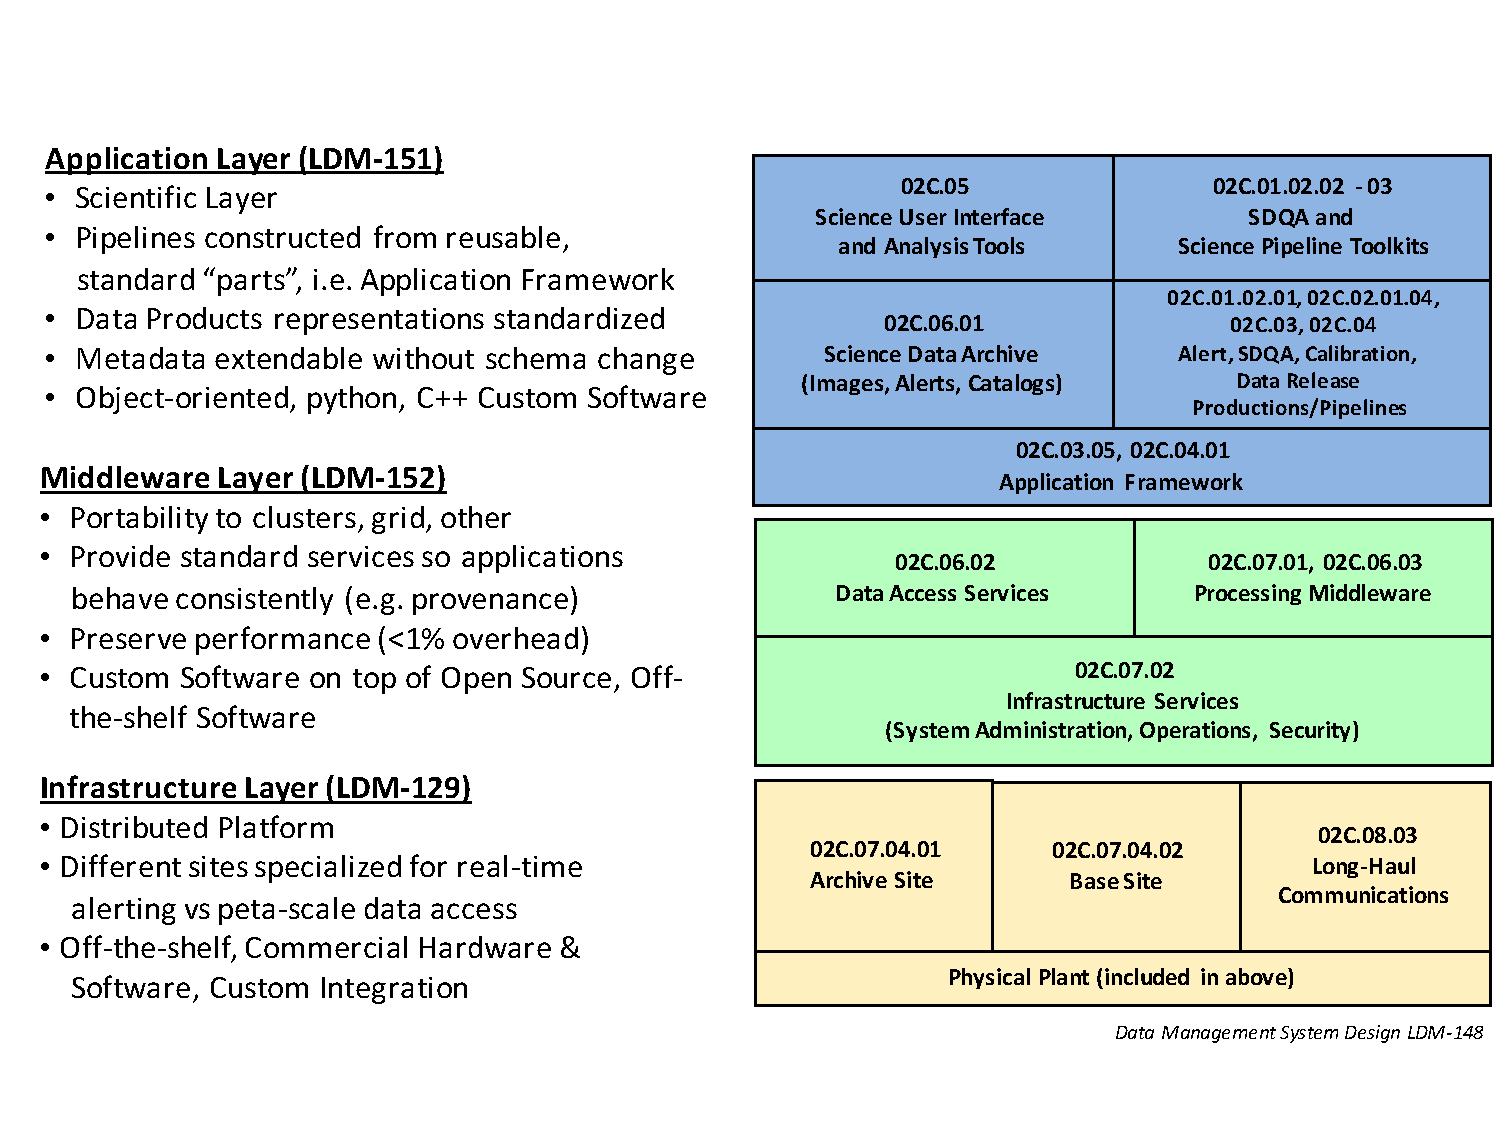
\includegraphics[angle=90,scale=0.70]{DMS-Architecture.pdf}
\caption{Architecture of the Data Management System\label{fig:DMS}}
\end{figure}

\begin{figure}
%\includegraphics[angle=90,scale=0.70]{ApplicationLayerProductionsandPipelines.eps}
\centering
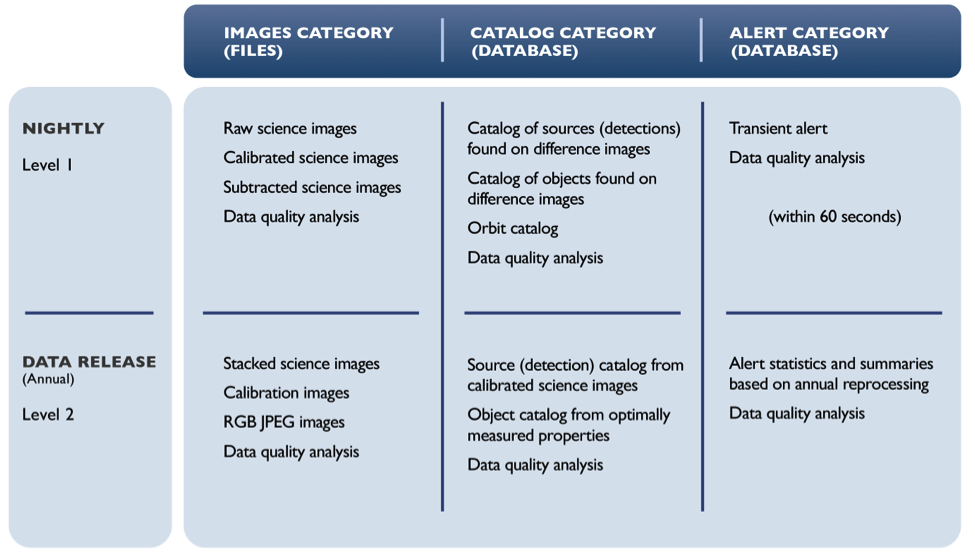
\includegraphics[angle=90]{DataProductDelivarables.png}
\caption{Organization of LSST Data Products\label{fig:DP}}
\end{figure}

\subsection{Data Products}

The LSST data products are organized into three groups, based on their intended use and/or origin. The full description is provided in the Data Products Definition Document (\DPDD); we summarize the key properties here to provide the necessary context for the discussion to follow. 

\begin{itemize}
\item {\bf Level 1} products are intended to support timely detection and follow-up
  of time-domain events (variable and transient sources). They are generated by
  near-real-time processing the stream of data from the camera system during 
  normal observing.  Level 1 products are therefore continuously generated and / or
  updated every observing night. This process is of necessity highly
  automated, and must proceed with absolutely minimal human
  interaction.  In addition to science data products, a number of related
  Level 1 ``SDQA''\footnote{Science Data Quality Analysis} data products are generated
  to assess quality and to provide feedback to the Observatory Control System (OCS).

\item {\bf Level 2} products are generated as part of a Data Release, generally
  performed 
  yearly, with an additional data release for the first 6 months of survey data. 
  Level 2 includes data products for which extensive
  computation is required, often because they combine information from
  many exposures.  Although the steps that generate Level 2 products
  will be automated, significant human interaction may be required at
  key points to ensure the quality of the data.

\item {\bf Level 3} products will be generated by the users of LSST, using LSST 
  software and/or hardware.  LSST DM is required to facilitate the creation of 
  Level 3 data products by providing suitable APIs, software components, and
  computing infrastructure, but will not by itself create any Level 3
  data product. Once created, Level 3 data products may be associated with 
  Level 1 and Level 2 data products through database federation.
  Where appropriate, the LSST Project, with the agreement of the Level 3
  creators, may incorporate user-contributed Level 3 data product pipelines
  into the DMS production flow, thereby promoting them to Level 1 or 2.

\end{itemize}
%
The organization of LSST Data Products is shown in Figure~\ref{fig:DP}.

Level 1 and Level 2 data products that have passed quality control
tests will be accessible to the public without restriction.
Additionally, the source code used to generate them will be made
available, and LSST will provide support for builds on selected
platforms.

\subsection{Science Pipelines Overview}

We recognize four major groups of science pipelines residing in the Applications layer:
\begin{itemize}
    \item {\bf Level 1 Pipelines}, grouped under the {\bf Alert Production} element of the WBS, are designed to generate Level 1 data products. These include:
    \begin{itemize}
    \item {\bf \emph{Single Frame Processing (``SFM'') Pipeline}} (\wbsSFM), to reduce acquired visits and detect and characterize astrophysical sources present in these visits.
    \item {\bf \emph{Image Differencing Pipeline}} (\wbsDiffim), to create difference images, and detect and characterize sources in them.
    \item {\bf \emph{Association Pipeline}} (\wbsAssocP), to associate sources detected in the difference images with known objects.
    \item {\bf \emph{Alert Generation Pipeline}} (\wbsAP), to generate and transmit alerts to time-domain events (e.g., transients) to the astronomical community, and
    \item {\bf \emph{Moving Object Pipeline}} (\wbsMOPS), to identify, link and compute orbits for Solar System objects detected in difference images.
    \end{itemize}
Level 1 pipelines run as the data are being acquired. They primarily focus on image differencing, and the reduction of information extracted from difference images. The algorithms they employ are designed and chosen to complete processing on minute (alert production) to day (Solar System object pipelines) time scales. They are also rerun as a part of Data Release Production (DRP), potentially in somewhat different configurations to achieve greater precision at the expense of increased runtime.
    
    \item {\bf Level 2 Pipelines} run annually or semi-annualy (for the first year of data), and are designed to generate deep co-adds and catalogs stemming from analysis of direct image data.  These include:
    \begin{itemize}
        \item {\bf \emph{PSF Estimation Pipeline}} (\wbsPSF), to estimate the PSF properties and variation across the focal plane for each visit, to the degree of precision required by the \SRD. Note that the work of this pipeline goes beyond the typical single-CCD PSF estimation present in the SFM pipeline.
        \item {\bf \emph{Image Coaddition Pipeline}} (\wbsCoadd), to generate and characterize coadded images of the sky, as well as create templates for image differencing.
        \item {\bf \emph{Object Detection and Deblending}} (\wbsDetDeblend), to detect sources in images of the sky and decompose them individual astronomical objects.
        \item {\bf \emph{Object Characterization Pipeline}} (\wbsObjChar), to characterize (perform measurements of) astrophysical objects detected in LSST imaging (both in single frames and coadds).
    \end{itemize}
    
    \item {\bf Calibration Pipelines} process the collected calibration data and perform calibration of LSST instruments and data products. These include:
    \begin{itemize}
        \item {\bf \emph{Calibration Products Pipeline}} (\wbsCPP), that generates the necessary calibration data products (e.g., master flats, biases, atmospheric models, etc.). It is run periodically as new calibration data are acquired.
        \item {\bf \emph{Photometric Calibration Pipeline}} (\wbsPhotoCal), that performs global photometric self-calibration of the Level 2 dataset.
        \item {\bf \emph{Astrometric Calibration Pipeline}} (\wbsAstroCal), that performs global astrometric self-calibration of the Level 2 dataset.
    \end{itemize}
    The calibration products pipeline is also rerun as a part of Data Release Processing. Global self-calibration steps run in DRP only.

       \item {\bf Science Data Quality Assessment (SDQA) pipelines and toolkits}, to enable collection, computation, visualization, monitoring and analysis of data quality metrics across all pipelines. These are divided into:
       \begin{itemize}
           \item {\bf \emph{Science Data Quality Assessment Pipeline}} (\wbsSDQAP), that provides low-level data collection functionality for SDQA and
           \item {\bf \emph{Science Data Quality Analyst Toolkit}} (\wbsSDQAT), that provides the visualization, analysis and monitoring capabilities for SDQA.
       \end{itemize}

\end{itemize}

In addition to these four, we recognize two other, cross-cutting, elements of DMS functionality:

\begin{itemize}
       \item {\bf \emph{Common Image and Catalog Processing framework}} (\wbsAFW), known as the {\bf Application Framework (afw)}, that collects base classes and algorithms % RHL need a better word than algorithms
         used by the DM Applications layer. The framework is split in two WBS elements, to reflect the multi-institutional nature of the work, but is functionally viewed as a single, integrated, component (class library).
       \item The {\bf \emph{Science Pipeline Toolkit}} (\wbsSPT), a collection of software components (and design principles) designed to enable construction of Level 3 pipelines relying on reusable lower-level components produced in support of other LSST DM software.
\end{itemize}

\subsubsection{Level 1 Pipelines Overview}
The production of Level 1 products is generally performed nightly, directly fed by 
the output data stream from the Camera SDS\footnote{Science Array Data Acquisition (DAQ) Subsystem} during observing. This data stream
contains both unprocessed (raw) camera images, and images that have been corrected
for crosstalk by the SDS on the Summit.  The normal observing
pattern is to take two 15 second exposures of the same field in immediate
succession.  These two exposures together form a {\em visit}, which is the typical
image data unit processed by the rest of the DM system.
\\

\begin{figure}
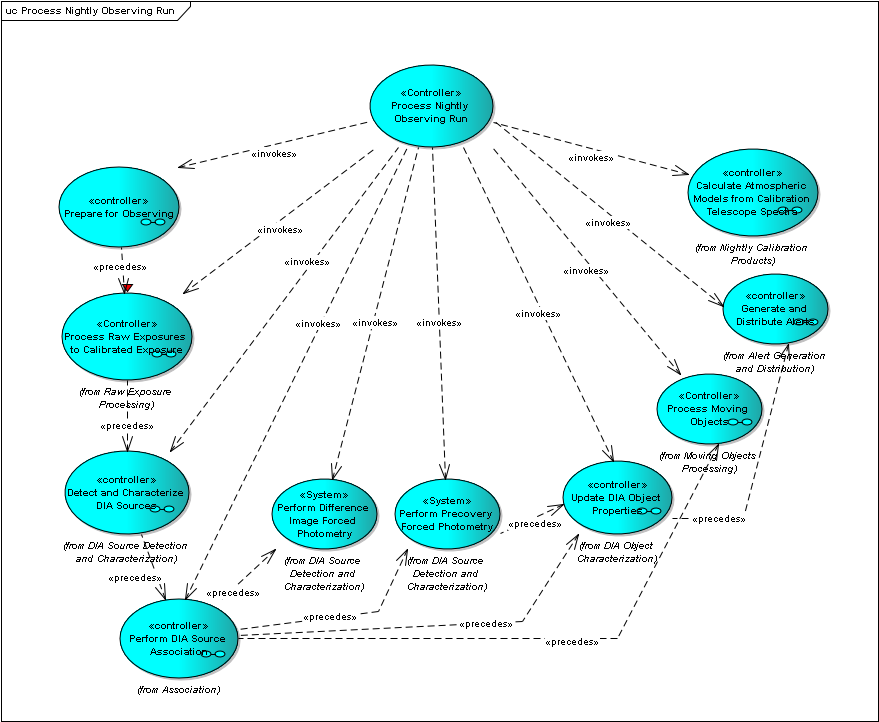
\includegraphics[angle=0,scale=0.44]{process_nightly_observing_run.png}
\caption{Level 1 Processing Flow Diagram\label{fig:level1}}
\end{figure}

The logical flow of Level 1 processing is shown in the Use Case diagram presented in Figure~\ref{fig:level1}. For every observation, the following sequence of events will unfold:
%
\begin{enumerate}
\item A visit is acquired (\uc{Prepare for Observing}) and reduced (\uc{Process Raw Exposures to Calibrated Exposure}) to a single {\em visit image}. This includes instrumental signature removal\footnote{E.g., subtraction of bias and dark frames, flat fielding, bad pixel/column interpolation, etc.}, combining of snaps, etc.
  % RHL I removed cosmic ray rejection as it's not clear if it's in ISR or snap combination.

\item The visit image is differenced against the appropriate template and \DIASources are detected (\uc{Detect and Characterize DIA Sources}). If necessary, deblending is performed at this stage.

The flux and shape of the DIASource are measured on the difference image. PSF photometry is performed on the visit image at the position of the \DIASource to obtain a measure of the absolute flux.
  % RHL this is tricky in crowded fields (inc. SNe on galaxies).  We should rethink this a bit at some point.

\item The \DB is searched for a \DIAObject or an \SSObject with which to positionally associate the newly discovered \DIASource. If no match is found, a new \DIAObject is created and the observed \DIASource is associated to it.

If the \DIASource has been associated to an \SSObject (a known Solar System object), it will be flagged as such and an alert will be issued. Further processing will occur in daytime (\uc{Process Moving Objects}).

\item Otherwise, the associated \DIAObject measurements will be updated with new data (\uc{Update DIA Object Properties}). All affected columns will be recomputed, including proper motions, centroids, light curves, nearest Level 2 \Objects, etc.
  % RHL do we really want to update e.g. the proper motion/parallax on each visit?

\item An alert is issued (\uc{Generate and Distribute Alerts}) that includes all required components, as described in the \DPDD.

\item For all \DIAObjects overlapping the field of view to which a \DIASource from this visit has \emph{not} been associated, forced photometry will be performed (\uc{Perform Difference Image Forced Photometry}).  No alerts will be issued for these measurements.

\end{enumerate}

Within 24 hours of discovery, LSST DM system will perform \emph{precovery} PSF forced photometry on any prior difference image overlapping the predicted position of new \DIAObjects taken within the past 30 days (\uc{Perform Precovery Forced Photometry}).
\\

Similarly, in daytime after the nightly observing run, atmospheric models from the calibration telescope spectra will be calculated (\uc{Calculate Atmospheric Models from Calibration Telescope Spectra}) and made available to the users.
\\

In addition to these, the Moving Object Pipeline (MOPS; \wbsMOPS; \uc{Process Moving Objects}) will also be run in daytime. It is described in its own section of this document, with a detailed design in a separate Moving Object Pipeline Design Document (\MOPSD).

\subsubsection{Level 2 Pipelines Overview}

\begin{figure}[!htbp]
    \centering
    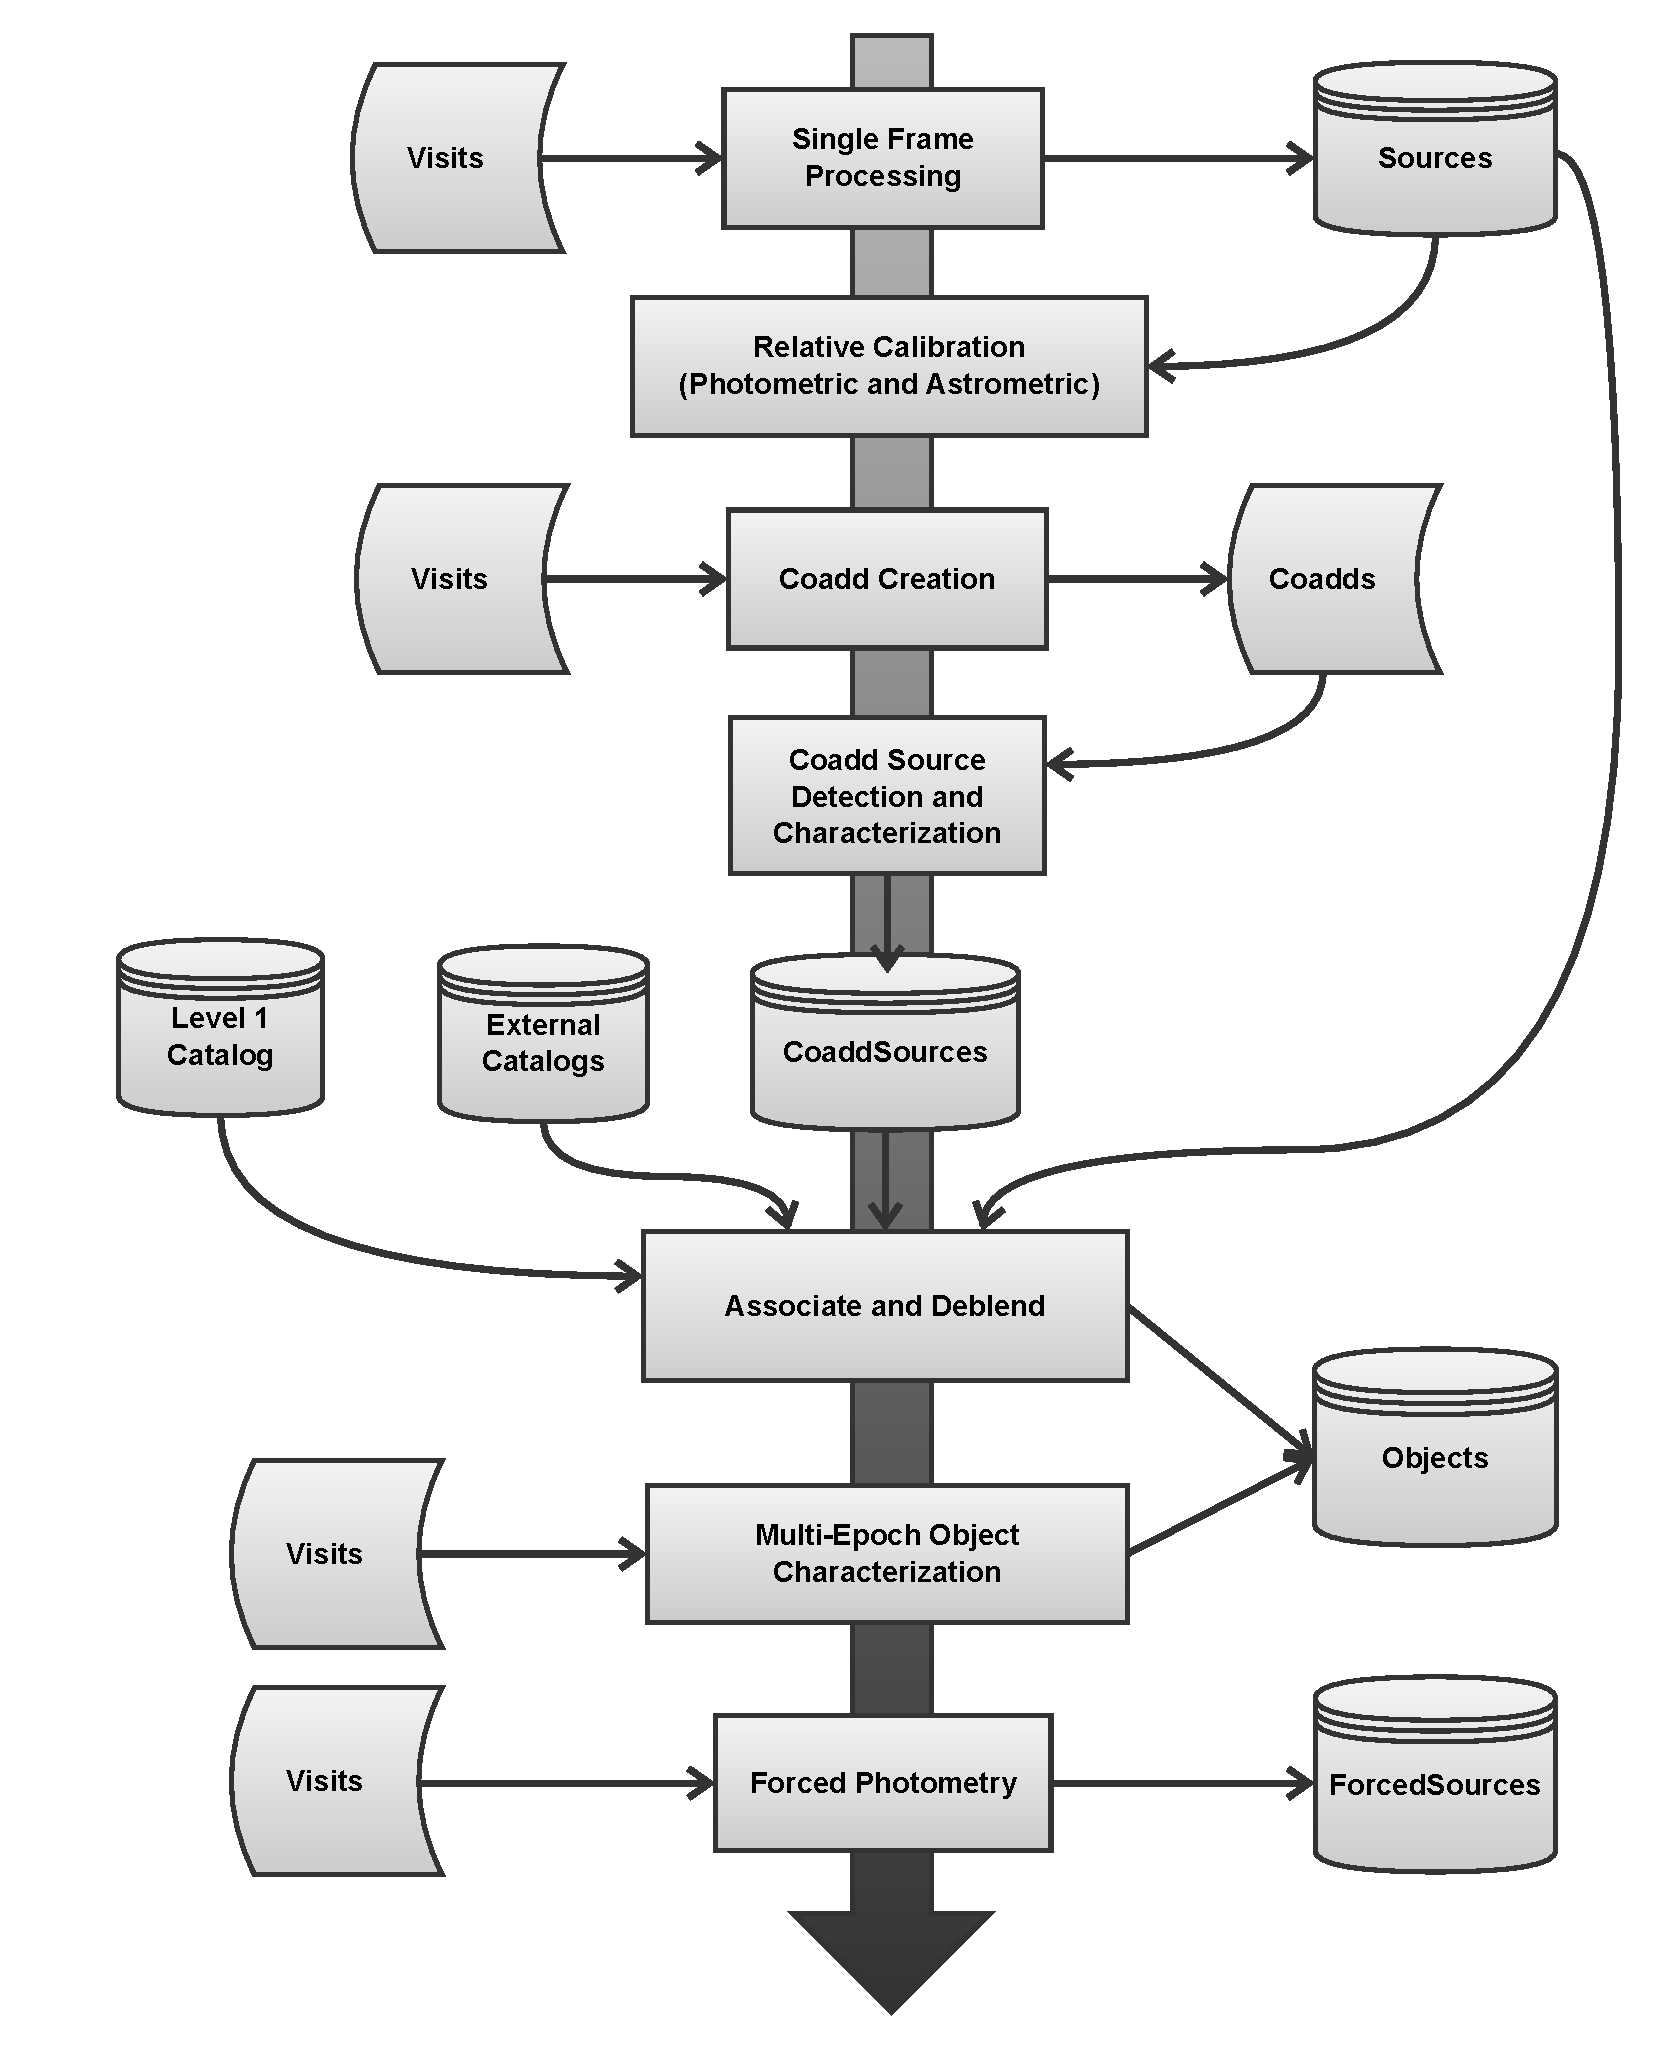
\includegraphics[scale=0.5]{Level_2_Processing_Flowchart}
    \caption{Level 2 Processing Overview\label{fig:level2dp}}    
\end{figure}

Figure~\ref{fig:level2dp} presents a high-level overview of the Level 2 data processing workflow. Logically\footnote{The actual implementation may parallelize these steps to the extent possible; see LDM-230, the Automated DM Operations Document (\DMOps).}, the processing begins with single-frame (visit) image reduction and source measurement, followed by global astrometric and photometric calibration, coadd creation, detection on coadds, association and deblending, object characterization, and forced photometry measurements. The UML Use Case model (\appsUMLusecase) captures these activities in the \uc{Produce a Data Release} diagram.
\\

The following is a high-level description of steps which occur during regular Level 2 data processing:
\begin{enumerate}
    \item \emph{Single Frame Processing}: Raw exposures are reduced to \emph{calibrated visit exposures}, and \Sources are independently detected, deblended, and measured on all visits. Their measurements (instrumental fluxes and shapes) are stored in the \Source table. This step is performed by the {\bf \emph{Single Frame Processing Pipeline}} (\wbsSFM).
    \item \emph{Relative calibration}: The survey is internally calibrated, both photometrically and astrometrically using the {\bf \emph{Astrometric}} (\wbsAstroCal) and {\bf \emph{Photometric Calibration Pipelines}} (\wbsPhotoCal). Relative zero points over the focal plane and astrometric corrections are computed for every visit.
    \item \emph{Coadd creation}: Deep, seeing optimized, and short-period per-band coadds are created in $ugrizy$ bands, as well as deeper, multi-color, coadds. This task is performed by the {\bf \emph{Image Coaddition Pipeline}} (\wbsCoadd). Transient sources (including Solar System objects, explosive transients, etc), will be rejected from the coadds.
    \item \emph{Coadd source detection}. Sources will be detected on all coadds generated in the previous step. The source detection algorithm will detect regions of connected pixels, known as \emph{footprints}, above the nominal $S/N$ threshold in the \emph{PSF-likelihood image} of the visit. Each footprint may have one or more \emph{peaks}, and the collection of these peaks (and their membership in the footprints) are the output of this stage. This information will be stored in a catalog of \CoaddSources. The detection is performed by the {\bf \emph{Object Detection and Deblending}} system (\wbsDetDeblend).
    \item \emph{Coadd source deblending and characterization}. The next stage in the pipeline will decompose the \CoaddSources into a set of individual astronomical sources which is consistent across all bands, a process known as \emph{deblending}. The deblender may make use of the catalogs of \Sources and \CoaddSources, catalogs of \DIASources, \DIAObjects and \SSObjects detected on difference images, and objects from external catalogs. The deblended objects will then be characterized by measuring their positions, shapes and fluxes on the coadded images and by fitting galaxy models. This functionality is contained within the {\bf \emph{Object Detection and Deblending}} system (\wbsDetDeblend) and the {\bf \emph{Object Characterization Pipeline}} (\wbsObjChar).
    \item \emph{Multi-epoch object characterization}. A set of measurements (including predefined classes of model fits) will be performed on each of the \Objects identified in the previous step, taking all available multi-epoch data into account. Model fits will be performed using \emph{MultiFit}-type algorithms. Rather than coadding a set of images and measuring object characteristics on the coadd, MultiFit simultaneously fits PSF-convolved models to the objects multiple observations. This reduces systematic errors, improves the overall $S/N$, and allows for fitting of time-dependent quantities degenerate with shape on the coadds (for example, the proper motion). The models we plan to fit will \emph{not} allow for flux variability. Object characterization is a part of the {\bf \emph{Object Characterization Pipeline}} (\wbsObjChar).
    \item \emph{Forced Photometry}. Source fluxes will be measured on every visit, with the position, motion, structural parameters, and deblending characterized in the previous step kept fixed.
      % RHL we're not clear about which model we'll use for this forced photometry. The best-fit Sersic? 
      This process of \emph{forced photometry}, will result in the characterization of the light-curve for each object in the survey. Forced photometry is functionally a part of the {\bf \emph{Object Characterization Pipeline}} (\wbsObjChar).
\end{enumerate}


% \subsubsection{Calibration Pipelines}

\subsubsection{Enabling Level 3 Pipelines}

Level 3 capabilities are envisioned to enable science cases requiring further custom user-specified processing, especially the kind that would greatly benefit from co-location within the LSST Data Access Center. The high-level requirement for Level 3 is established in \S 3.5 of the LSST SRD.

To enable Level 3 use cases, LSST Data Management pipelines will be designed in a modular fashion to maximize the potential for reusability and synergy between Level 3 and Levels 1 and 2.

For example, a typical Level 3 use case will be to perform a different kind of measurement on objects detected in the course of Level 2 processing. A user will be able to do this by reusing the desired components of Level 2 processing, plugging in (via Python {\tt import} directives in the appropriate configuration file) the modules for their custom measurement, and executing the pipeline. The {\bf \emph{Science Pipeline Toolkit}} (\wbsSPT) will provide the necessary components to support user-driven construction and execution of custom pipelines.

\subsubsection{Science Data Quality Analysis Pipeline and Toolkit}

Science Data Quality Analysis requirements are described in the Data Quality Assurance Plan (\SDQAP) document. They will be implemented by the {\bf \emph{SDQA Pipeline}} (\wbsSDQAP; the data collection backend) and the {\bf \emph{SDQA Toolkit}} (\wbsSDQAT; the data analysis front-end).
\\

LSST QA will include four main components, which to some extent reflect the Level 1-3 structure of LSST data products. Level 0 QA is software development related, Level 1 QA relates to nightly operations, Level 2 QA relates to data releases, and Level 3 QA is science based.

\begin{itemize}
    \item {\bf Level 0 QA} includes the extensive and thorough testing of the DM subsystem during the pre- commissioning phase, as well as the tests of software improvements during the commissioning and operations phases (regression tests based on pipeline outputs and input truth). A common feature of Level 0 QA is the use of LSST simulations products, or any other dataset where the truth is sufficiently well known (e.g., the use of high-resolution observations from space telescopes to test resolved/unresolved object separation algorithms). The main goal of Level 0 QA is to quantify the software performance against these known expected outputs (e.g., to measure the completeness and false positive rate for an object finder; to measure the impact of blended sources on pipeline outputs; to measure the performance of calibration pipelines and MOPS), and to test for algorithm implementation problems (a.k.a. “coding bugs”).
    
    \item {\bf Level 1 QA} assesses the system status and data quality in real time during commissioning and operations. Its main difference from other observatory, telescope, and camera status reporting tools will be heavy reliance on the massive science imaging data stream (in addition to various telemetry and metadata generated by the subsystems). This level is tasked with nightly reporting of the overall data quality, including the nightly data products (difference images and transient source event stream) and calibration products. Real-time information about observing conditions, such as sky brightness, transparency, seeing, and about the system performance, such as the achieved faint limit, will be delivered by Level 1 QA\@. Because the actual science data stream will be analyzed, Level 1 QA tools will be in a good position to discover and characterize subtle deterioration in system performance that might not be easily caught by tools employed by the telescope and the camera subsystems for self-reporting purposes.

    \item {\bf Level 2 QA} assesses the quality of data products scheduled for the Data Releases, and provides quantitative details about data quality for each release (including the co-added image data products, and the properties of astrometrically and photometrically variable objects). This level also performs quality assessment for astrometric and photometric calibration, as well as for derived products, such as photometric redshifts for galaxies
      % RHL are we responsible for photo-z quality?  I thought it was Level 3
      and various photometric estimators for stars. Subtle problems with the image processing pipelines and systematic problems with the instrument will be discovered with Level 2 QA.
    
    \item {\bf Level 3 QA} quality assessment will be based on science analysis performed by the LSST user community. LSST will not develop Level 3 QA tools, but Level 0-2 visualization and data exploration tools will be made available to the community to form a basis on which Level 3 tools can be built. Common features expected for tools at this level are sensitivity to subtle systematic issues not recognized by Level 2 QA, and feedback about data quality to the project by external teams. It is envisioned that especially useful Level 3 QA tools would be migrated to Level 2 QA.

\end{itemize}

\clearpage

\section{Shared Software Components}

\subsection{Applications Framework (\wbsAFW)}

\subsubsection{Key Requirements}

The {\bf \emph{LSST Applications Framework}} ({\tt afw}) is to provide the basic functionality needed by an image processing system. In particular, it shall provide:
%
\begin{itemize}
    \item Classes to represent and manipulate mappings between device and astronomical coordinates.
    \item Classes to represent and manipulate images and exposures\footnote{images with associated metadata.}
    \item Classes to represent and estimate backgrounds on images
    \item Classes to represent the geometry of the camera
    \item Base classes to represent and manipulate the point spread function (PSF)
    \item Routines to perform detection of sources on images, and classes to represent these detections (\emph{``footprints''})
    \item Classes to represent astronomical objects
    \item Classes to represent and manipulate tables of astronomical objects
    \item Other low-level operations as needed by LSST science pipelines 
\end{itemize}

\subsubsection{Baseline design}

\begin{figure}
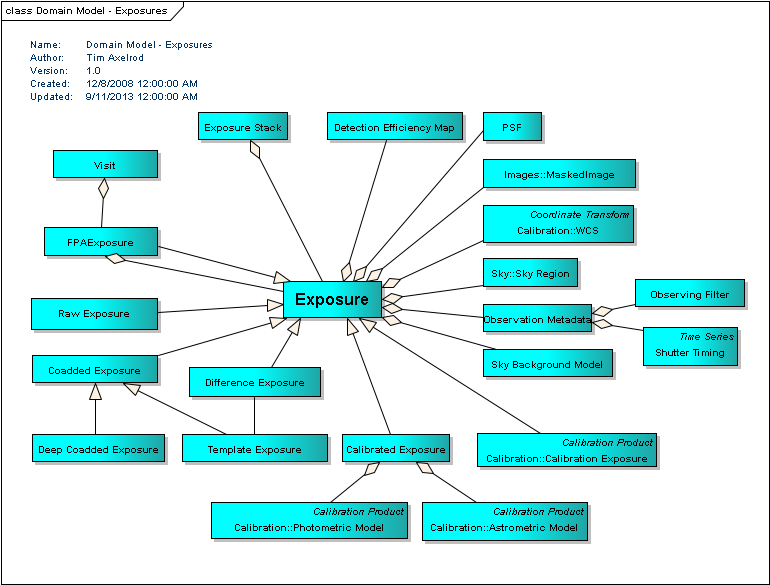
\includegraphics[angle=0,scale=0.54]{domain_model_-_exposures.png}
\caption{Exposure class diagram\label{fig:exposureUML}}
\end{figure}

The baseline design calls for a library of C++ classes and functions, exposed to Python callers as a Python module named {\tt lsst.afw}. The classes required are captured in the UML Domain Model (\appsUMLdomain), with an example of the Exposure class shown in Figure~\ref{fig:exposureUML}.
\\

This library will form the basis for all image processing pipelines and algorithms used for LSST so special attention will be paid to performance.

% \subsubsection{Constituent Use Cases and Diagrams}

\subsubsection{Prototype Implementation}

A prototype implementation of the baseline design has been completed in LSST Final Design Phase, including prototype GPU (CUDA) support for major image processing functions (e.g., warping). We expect it will be possible to transfer a significant fraction of the existing code into Construction.
\\

Needs for future improvement have been identified in three areas:
\begin{itemize}
    \item The current design of classes that represent the Camera geometry is suboptimal. Redesign will be needed in Construction.
    \item The current design of classes that represent the PSF does not allow for intensity-dependent PSF terms. These will need to be added in construction.
    \item Design of sky background and geometry classes was found to be insufficiently flexible. This will need to be rectified in Construction.
\end{itemize}
% RHL I can think of lots more...

Prototype code is available at \url{https://github.com/lsst/afw/}. The documentation for the prototype is located at \url{http://ls.st/w3o} and \url{http://ls.st/6i0}.

\clearpage

\section{Level 1 Pipelines}

\subsection{Single Frame Processing Pipeline (\wbsSFM)}

\subsubsection{Key Requirements}

Single Frame Processing (SFM) Pipeline is responsible for reducing raw image data to \emph{calibrated exposures}, and detection and measurement of \Sources (using the components functionally a part of the Object Characterization Pipeline).
\\

SFM pipeline functions include:
%
\begin{itemize}
    \item Assembly of per-amplifier images to an image of the entire CCD;
    \item Instrumental Signature Removal;
    \item Cosmic ray rejection and snap combining;
    \item Per-CCD Determination of zeropoint and aperture corrections;
    \item Per-CCD PSF determination;
    \item Per-CCD WCS determination and astrometric registration of images;
    \item Per-CCD sky background determination;
    \item Source detection.
\end{itemize}

Calibrated exposure produced by the SFM pipeline must possess all information necessary for measurement of source properties by single-epoch Object Characterization algorithms.

It shall be possible to run this pipeline in two modes: a ``fast" mode needed in nightly operations for Level 1 data reductions where no source characterization is done beyond what's required for zero-point, PSF, sky, and WCS determination (image reduction); and a ``full" mode that will be run for Level 2 data reductions.

\subsubsection{Baseline design}

Single Frame Processing pipeline will be implemented as a flexible framework where different data can be easily treated differently, and new processing steps can be added without modifying the stack code.
\\

It will consist of three primary components:
%
\begin{itemize}
    \item A library of useful methods that wrap a small number of atomic operations (e.g., {\tt interpolateFromMask}, {\tt overscanCorrection}, {\tt biasCorrection}, etc.) % RHL things like overscanCorrection aren't atomic (or at least, they use afw::math and afw::cameraGeom primitives)
    \item A set of classes ({\tt Task}s) that perform higher level jobs
    (e.g., {\tt AssembleCcdTask}, or {\tt FringeTask}), and a top level class to apply corrections to the input data in the proper order. This top level class can be overridden in the instrument specific {\tt obs\_*} packages, making the core SFM pipeline camera agnostic.
    \item A top-level Task to run the SFM pipeline.
\end{itemize}

In the paragraphs to follow, we describe the adopted baseline for key SFM algorithms. If not discussed explicitly, the algorithmic baseline for all other functionallity is assumed to be the same as that used by SDSS \emph{Photo} pipeline \cite{LuptonPhoto}.

\paragraph{Instrumental Signature Removal:}

The adopted pipeline design allows for straightforward addition of correction for instrumental effects that will be discovered in the as-built Camera. The effects currently baselined to be corrected are:

\begin{itemize}
\item Bias: A master bias frame, created from a set of overscan corrected zero length exposures, is subtracted from the image to correct for 2D structure in the bias level. For each exposure, overscan columns will be averaged and fit with a 1D function and subtracted row by row to account for time variable bias level.

\item Assembly: CCDs will be assembled by trimming the prescan and/or overscan rows and columns from amplifier images and storing them into a Image object.

\item Dark current: A master dark frame created from a set of bias corrected exposures taken with the shutter closed is scaled to the science image exposure time and subtracted to correct for 2D structure in the dark current.

\item Cross-talk: Cross talk is generated by interaction of fields produced by the current in physically proximate electronic components. This results in bright features from one amp showing up in other. Correction is to subtract each aggressor amp (possibly flipped) modulated by a measured coefficient from the victim amp. The implementation may assume the cross-talk is small enough to be correctable by first order correction only.

\item Non-linearity: CCDs do not have perfectly linear response. At both almost empty and almost full well the response can become non-linear. Given a measurement of the linearity of the CCD response, along with any temperature dependence, the data values will be corrected to linear response by simple mapping and interpolation.

\item Flat-field: The correction is a division by the normalized master flat. The master flat will be generated assuming a nominal flat spectrum for all sources. Photometric corrections will be applied downstream on a source by source basis given an SED for each source.

\item Fringing: Fringe parerns are an interference effect that result from the sharp emission lines in the night sky spectrum. This effect is the strongest in redder bands. The best fit modeled fringe pattern, constructed from monochromatic flats assuming a low-dimensional parametrization of the night sky emission spectrum, will be subtracted from the image.

\item Cosmic ray rejection and snap combining: Exposures will be taken in pairs separated by the readout time. The two images and the expected statistics on those images are used to reject pixels that are significant outliers. Once cosmic rays are flagged the two snaps will be added to produce an image with a longer effective exposure.  % RHL There'll probably also be a significant morphological component.  Esp. if we want snap-to-snap transients...
\end{itemize}

\paragraph{PSF determination:} We will run separate algorithms to select candidate stars and determine the point-spread function (PSF, the light distribution for a point source, a critical ingredient to understanding the data and measuring accurate fluxes and shapes).  Both the star selector and PSF determiner algorithms will be pluggable Python modules, so that different algorithms can be run as desired for different analysis needs.

Three selectors will be implemented. % RHL I bet that these will change dramatically before construction.  I was tempted to change ``will be implemented'' to ``will be implemented initially'' but didn't.
The ``second-moment'' star selector will builds a histogram of the X and Y second moments of flux, search for a peak, and select sources in the peak as point source candidates.  The ``catalog'' star selector, in contrast, will make use of an external catalog of point sources and use astrometric matching to select point source candidates.  The ``objectSize'' star selector will identify point source candidates from the cluster of sources with similar sizes regardless of magnitude.  When selecting point source candidates by size (i.e., for the ``second-moment'' and ``objectSize'' algorithms), the sizes will be corrected by the known optical distortion of the camera.  % RHL objectSize has superceded secondMoment already.
\\

Given the irregularly sampled grid of PSFs represented by selected stars, the variation of the PSF across the CCD will be determined. The baselined ``principal-components'' PSF (pcaPsf) determiner performs a singular value decomposition (also known as a principal components analysis, or PCA) on the point-source candidates in pixel space to produce a set of eigen-images.  Using the dominant eigen-images, it constructs polynomial interpolants for their relative weights.  This produces a spatially-varying PSF model that captures the most important changes in the PSF over the CCD.
\\

These algorithms are intended to be sufficient to enable Level 1 processing. More advanced PSF determination algorithms will be developed in the PSF Estimation Pipeline (\wbsPSF).
% RHL We'll have to be careful, as I think these fluxes/positions are the inputs into global calibration

\paragraph{Sky Background Determination:}

We will estimate the smooth sky background by measuring the background level in cells (typically 256 or 512 pixels square) % RHL I'm sure 256 will be too small.  512 may well be too.
using (by default) a clipped mean, and ignoring pixels that are part of detected sources.  An interpolating spline (an Akima spline, by default) will be constructed to estimate the background level in each pixel. Backgrounds will be possible to estimate simultaneously over multiple sensors, including the full focal plane.

Background models will be saved, for later subtraction or restoration (e.g., in background matching, as implemented by the Coaddition Pipeline, \wbsCoadd).

\paragraph{WCS determination and image registration}

The absolute World Coordinate System (WCS) will be determined using an \emph{astrometry.net} type algorithm \cite{Lang09}, seeded with the approximate position of the boresight.  % RHL I doubt if we'll use a.n in production (except as a fallback when all else fails)

This module will also include the capability to perform relative registration of a set of images to enable coaddition and image differencing, using the \emph{meas\_mosaic} registration algorithm developed by Furusawa et al. \cite{Furusawa14} as the baseline.

\subsubsection{Constituent Use Cases and Diagrams}

Assemble CCD; Determine Aperture Correction; Determine PSF; Remove Instrument Signature; Detect Sources; Determine Photometric Zeropoint; Measure Single Visit Sources; Determine WCS; Sum Exposures, Combine Raw Exposures, Remove Exposure Artifacts; Determine Sky Background Model; Calibrate Exposure; Process Raw Exposures to Calibrated Exposure; Perform Single Visit Processing;

\subsubsection{Prototype Implementation}

A prototype implementation of all major components of SFM baseline design has been completed in LSST Final Design Phase. The achieved accuracy is comparable to state-of-the art codes today (e.g., SDSS, SExtractor). We expect it will be possible to transfer a significant fraction of the existing code into Construction, with continued improvement to meet LSST accuracy requirements.
\\

WCS determination and image registration modules are an exception, and will require extensive redesign and rewrite. The sky determination module will have to be enhanced to support multi-CCD fitting capability.
\\

The prototype codes are available in the following repositories: \url{https://github.com/lsst/ip_isr}, \url{https://github.com/lsst/meas_algorithms}, \url{https://github.com/lsst/meas_astrom}, \url{https://github.com/lsst-dm/legacy-meas_mosaic}, \url{https://github.com/lsst/pipe_tasks}.

\clearpage

\subsection{Image Differencing Pipeline (\wbsDiffim)}

\subsubsection{Key Requirements}

The image differencing pipeline shall difference a visit image against a deeper template, and detect and characterize sources in the difference image in the time required to achieve the 60 second design goal for Level 1 alert processing (current timing allocation: 24 seconds). The algorithms employed by the pipeline shall result in purity and completeness of the sample as required by the \DMSR\@. Image differencing shall perform as well in crowded as in uncrowded fields.

\subsubsection{Baseline design}

\begin{figure}
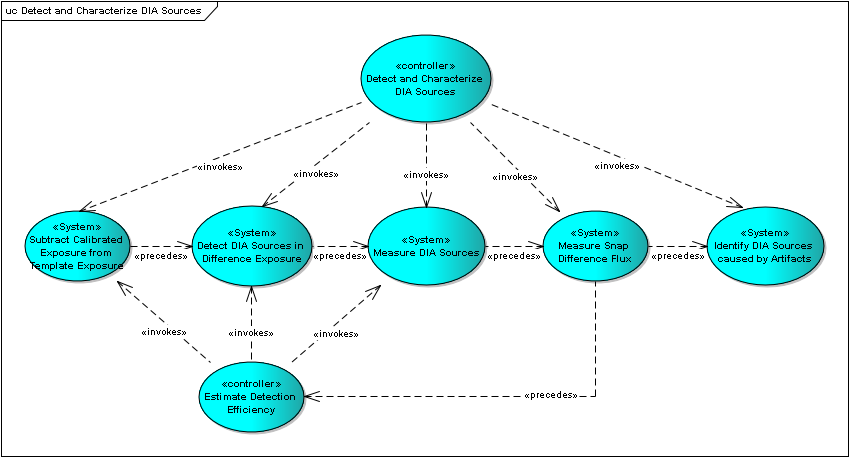
\includegraphics[angle=0,scale=0.44]{detect_and_characterize_dia_sources.png}
\caption{Image Differencing Pipeline Use Case Diagram\label{fig:diffimUML}}
\end{figure}

The Image Differencing pipeline will difference, detect, and deblend objects in the resulting image using the ``preconvolution'' algorithm as described in Becker et al. (\url{http://ls.st/x9f}).
Differencing will be performed against a deeper template, and differential chromatic refraction (DCR) will be handled by having templates in several bins of airmass.

All \DIASource measurements described in the \DPDD, including post-processing such as variability characterization, will be performed for all sources detected in this manner. The measurements will be performed on the pre-convolved likelihood image. The measurement code will reside in a separate module in the Object Characterization Pipeline (\wbsObjChar).
\\

If necessary a \emph{spuriousness metric} using machine-learning techniques (e.g., Bloom et al. \cite{Bloom12}) will be developed to help in the discrimination of real sources from those caused by artifacts.
\\

Details of this baseline design have been captured in the \uc{Detect and Characterize DIA Sources} and related diagrams, presented in Figure~\ref{fig:diffimUML}.

\subsubsection{Constituent Use Cases and Diagrams}

Subtract Calibrated Exposure from Template Exposure; Identify DIA Sources caused by Artifacts; Perform Precovery Forced Photometry; Measure DIA Sources; Detect DIA Sources in Difference Exposure; Measure Snap Difference Flux; Perform Difference Image Forced Photometry; Calculate DIA Object Flux Variability Metrics; Fit DIA Object Position and Motion;

\subsubsection{Prototype Implementation}

A prototype implementation partially implementing the baseline design has been completed in the LSST Final Design Phase. It includes detection, centroiding, aperture and PSF photometry, and adaptive shape measurement.
% RHL I don't think it does, or at least not correctly.  I think that they just ran the standard algorithms as black boxes rather than adjusting them allow for the preconvolution.
This implementation was used to benchmark the speed of the image differencing code and examine the expected levels of false positives. Deblending on difference images, fits to trailed sources, and dipole fits were not prototyped. The final report on prototype design and performance can be found in Becker et al. (\url{http://ls.st/x9f}).
\\

The prototype code is available at \url{https://github.com/lsst/ip_diffim}. The current prototype, while functional, will require a partial redesign to be transfered to construction to address performance and extensibility concerns.

\clearpage

\subsection{Association Pipeline (\wbsAssocP)}

\subsubsection{Key Requirements}

The Association Pipeline has two key responsibilities: i) it must be able to associate newly discovered \DIASources with previously known \DIAObjects and \SSObjects, and ii) it must be able to associate \DIAObjects with known \Objects from the Level 2 catalogs.

\subsubsection{Baseline design}

The baseline design for \DIASources to \DIAObject association and \DIAObject to \Object association is to use simple nearest-neighbor search while taking proper motions and positional errors ellipses into account.

For matches to \SSObjects, the \SSObject's ephemeris are to be computed by NightMOPS (functionally a part of the Moving Object Pipeline, \wbsMOPS). Matching to the computed ephemeris is to be performed as if they were \DIAObjects.

When Level 1 data is reprocessed, a more sophisticated clustering algorithm \cite{Ankerst99} will be employed.

\subsubsection{Constituent Use Cases and Diagrams}

Create Instance Catalog for Visit; Associate with Instance Catalog;
Perform DIA Object Association; Perform DIA Source Association;

\subsubsection{Prototype Implementation}

Prototype implementation of the baseline design has been completed in LSST Final Design Phase. The nearest-neighbor matching has been implemented as a part of the Application Framework, while clustering using OPTICS resides in the database-related ingest modules.
\\

The prototype code is available at \url{https://github.com/lsst/ap}. The current prototype, while functional, will require a partial redesign in Construction to address scalability and performance.

\clearpage

\subsection{Alert Generation Pipeline (\wbsAP)}

\subsubsection{Key Requirements}

Alert Generation Pipeline shall take the newly discovered \DIASources and all associated metadata as described in the \DPDD, and generate alert packets in \VOEvent format. It will transmit these packets to VO Event Brokers, using standard IVOA protocols (eg., VOEvent Transport Protocol; VTP\@. End-users will primarily use these brokers to classify and filter events for subsets fitting their science goals.
% RHL I thought that we were being careful to say we'll use whatever's the standard, e.g. VO?

To directly serve the end-users, the Alert Generation Pipeline shall provide a basic, limited capacity, alert filtering service. This service will run at the LSST U.S. Archive Center (at NCSA). It will let astronomers create simple filters that limit what alerts are ultimately forwarded to them. These \emph{user defined filters} will be possible to specify using an SQL-like declarative language, or short snippets of (likely Python) code.

\subsubsection{Baseline design}

The baseline design is to adopt and upgrade for performance and functionallity the Skyalert package (\url{http://lib.skyalert.org/skyalert/}).

\subsubsection{Constituent Use Cases and Diagrams}

Distribute to Subscribed Brokers; Distribute to Subscribed Users; Generate Alerts;
Generate and Distribute Alerts;

\subsubsection{Prototype Implementation}

No prototype implementation has been developed by LSST, as the Skyalert package (\url{http://lib.skyalert.org/skyalert/}) was found to be mature enough to baseline the architecture and estimate costs.

\clearpage

\subsection{Moving Object Pipeline (\wbsMOPS)}

\subsubsection{Key Requirements}

The Moving Object Pipeline System (MOPS) has two responsibilities within LSST Data Management:

\begin{itemize}
    \item First, it is responsible for generating and managing the Solar System\footnote{Also sometimes referred to as `Moving Object'} data products. These are Solar System objects with associated Keplerian orbits, errors, and detected \DIASources. Quantitatively, it shall be capable of detecting 95\% of all Solar System objects that meet the findability criteria as defined in the \OSS\@. The software components implementing this function are known as {\bf \em DayMOPS}.
    \item The second responsibility of the MOPS is to predict future locations of moving objects in incoming images so that their sources may be associated with known objects; this will reduce the number of spurious transient detections and appropriately flag alerts to detections of known Solar System objects.  The software components implementing this function are known as {\bf \em NightMOPS}.
\end{itemize}

\subsubsection{Baseline design}

The baseline NightMOPS design is to adopt and adapt an existing ephemeris computation pipeline such as OrbFit\footnote{\url{http://adams.dm.unipi.it/orbfit/}} or OpenOrb\footnote{\url{https://github.com/oorb/oorb}}. The baseline DayMOPS design uses Kubica et al. \cite{Kubica05} algorithms to identify and link Solar System object candidates.
\\

The design of these components are explained in detail in the MOPS Design Document (\MOPSD).

\subsubsection{Constituent Use Cases and Diagrams}

Process Moving Objects;
Fit Orbit; Prune Moving Object Catalog; Perform Precovery; Recalculate Solar System Object Properties; Link Tracklets into Tracks; Find Tracklets;

\subsubsection{Prototype Implementation}

A prototype implementation implementing the key components of DayMOPS baseline design has been completed in LSST Final Design Phase. NightMOPS has not been extensively prototyped, as it is understood not to be an area of significant uncertainty and risk. An extensive report on MOPS prototyping and performance is available as a part of the MOPS Design Document (\MOPSD).
\\

Prototype MOPS codes are available at \url{https://github.com/lsst/mops_daymops} and \url{https://github.com/lsst/mops_nightmops}. We expect it will be possible to transfer a significant fraction of the existing code into Construction. Current DayMOPS prototype already performs within the computational envelope envisioned for LSST Operations, though it does not yet reach the required completeness requirement.

\clearpage

\section{Level 2 Pipelines}

\subsection{PSF Estimation Pipeline (\wbsPSF)}

\subsubsection{Key Requirements}

PSF Estimation pipeline must enable the estimation of the point spread function with residual ellipticity correlations at the levels required by LSR-REQ-0097.

\subsubsection{Baseline design}

LSST's PSF models will be implemented as a plugin. Simple PSF estimation algorithms (e.g., {\tt pcaPsf}) will be implemented by the Single Frame Processing pipeline (\wbsSFM). The CoaddPsf algorithm will be implemented in the Image Coaddition Pipeline (\wbsCoadd).
\\

Current state-of-the-art PSF estimation methods typically use some basis functions (e.g., $\delta$-functions, PCA) and a spatial model (e.g., polynomials) to estimate the PSF\@. This is not expected to be sufficient to reach LSST requirements. We've therefore adopted a baseline algorithm as follows:
\begin{itemize}
    \item Decompose the PSF into a component due to the atmosphere and a component due to the telescope and camera system.
    \item Estimate the telescope+camera component using the wavefront sensor information (the reconstructed wavefront) and camera metrology (the laboratory or on-sky measurement of $z$ offsets of individual sensors)
    \item Estimate the atmospheric contribution by modelling the PSF from bright, isolated, stars, and interpolating using Kriging. % RHL PCA \'a la Jarvis and Jain only works for the camera part
\end{itemize}
This estimation will be performed on the full focal plane, and use the per-CCD estimates of the PSF and cutouts of bright stars (PSF estimation candidates) as inputs.
\\
The PSF of thick deep depletion devices such as LSST's is known to be intensity dependent. We will estimate the zero-intensity PSF by iteratively forward-modeling the estimated zero-intensity PSF until convergence is achieved. The same forward-modelling algorithm will allow us to estimate the PSF in undersampled imaging, as is expected for roughly the best quartile of the seeing distribution.
% RHL [As you know] it's more accurate to say that the as-detected image is an intensity-dependent mapping of the image incident on the CCD (I must be able to find a better way to express that!).  A consequence is that the PSF is intensity dependent.

\subsubsection{Constituent Use Cases and Diagrams}

Perform Full Focal Plane PSF Estimation;

\subsubsection{Prototype Implementation}

Prototype code for wavefront reconstruction has been developed by the LSST Telescope and Site group. We expect this code will be rewritten in Construction to follow LSST Data Management standards and be straightforward to incorporate into the PSF Estimation pipeline.
\\

The remaining components of the PSF Estimation pipeline have not been prototyped at this time.

\clearpage

\subsection{Image Coaddition Pipeline (\wbsCoadd)}

\subsubsection{Key Requirements}

Image Coaddition Pipeline will produce coadds given a stack of input calibrated exposures. Generated coadds must be characterized, at a pixel level, for validity and variance (i.e., have a Mask plane and a Variance plane). It must be capable of supporting these coaddition schemes within a single band:
\begin{itemize}
    \item{Direct;}
    \item{PSF-matched;}
    \item{Likelihood (``Kaiser'').}
\end{itemize}

It must be capable of combining coadds from mulitple bands into a single, multi-band, coadd. When doing so, it must support both the ``$\chi^2$'' scheme described by \cite{Szalay99} and scheme in which inputs are weighted by the expected SED.

When non-PSF-matched coadds are produced, the effective PSF and its variation across the full coadd must be determined and retained. Outliers appearing in a small subset of input images (e.g., transients or moving objects) must not appear in the final co-adds. % RHL how we handle variables (e.g., RR Lyrae's) is not obvious

The Image Coaddition Pipeline must make it possible to generate the coadds with astrophysical backgrounds removed or retained, depending on runtime configuration directives.

The pipeline must be capable of generating coadds in varying geometries and tessellations of the sky, plugged in at runtime via Python modules and configuration directives. To reduce its memory footprint, it should be capable of generating the coadds in small patches set by the operator at runtime via configuration directives.

The pipeline should be capable of co-adding undersampled images without aliasing.

For performance reasons, the pipeline should be able to simultaneously generate multiple coadds from the same input stack, avoiding unnecessary rewarping of inputs to generate each coadd.

\subsubsection{Baseline design}

\paragraph{Coaddition}
\label{alg:coadd}

The Coaddition Pipeline will apply the results of the relative astrometric solution (developed as a part of Single Frame Pipeline, \wbsSFM) to the input images, warp (\S\ref{alg:warp}) them to a common coordinate system (``sky map''; \S\ref{alg:skymap}) and coadd the pixels. The warped images will be kept in memory. Using those images, multiple coadds will be created, each consisting of a subset of input images defined explicitly by the operator or algoritmically by quality cuts.

To accurately measure the colors of galaxies (e.g., for photometric redshifts) in the presence of intra-object color gradients, seeing changes and imperfect galaxy models, the baseline implementation will be capable of producing ``PSF-matched coadds'' using well known PSF-matching algorithms. The Object Characterization Pipeline (\wbsObjChar) will measure object properties on both direct (centroids and shapes) and PSF-matched (fluxes) coadds, as well as fitting galaxy models to the direct coaads.

Likelihood coaddition presents a possible alternative to direct and PSF-matched coaddition for both detection and measurement. Assessing the suitability of likelihood coadds for use in LSST data releases is contained within the Object Characterization Pipeline (\wbsObjChar); the Image Coaddition Pipeline will deliver likelihood coadds as required to satisfy that requirement.

The Detection and Deblending system (\wbsDetDeblend) will make use of multi-band coadds. These may be generated either using the $\chi^2$ algorithm \cite{Szalay99} or based on SED-weighted combinations of per-band coadds. The Image Coaddition Pipeline will make it possible to generate either of these on demand.

If the seeing is not constant it becomes impossible to produce a coadd with a PSF varying in a continuous fashion over the field, unless the data is deliberately degraded by convolving the inputs to a common PSF (known as ``PSF matching").  In order to enable dealing with the discontinuous PSF, the Coaddition Pipeline will construct a ``CoaddPsf'' (\S\ref{alg:coaddPsf}) PSF model, which is a sum of the PSFs of the input images at each point of interest (as proposed as part of `StackFit' \cite{Jee13}).

Determining the background from individual visits separately is problematic (because different choices can be made in each, especially at the edge of a CCD; and because extended, faint astrophysical flux is misinterpreted as background), commonly manifesting as dark rings around very bright stars and the suppression of extended flux around galaxies. Therefore, the pipeline will include the capability to perform ``background matching'' (\S\ref{alg:backgroundMatching}) to produce a coadd with a high signal-to-noise realization of the background in a single reference exposure.  This background will be measured over large scales and be possible to subtract with a high degree of accuracy. Background matching will be the default mode of operation. Nevertheless, it will also be possible to produce coadds by subtracting the background first using Sky Background determination and substraction components developed in the Single Frame Processing Pipeline (\wbsSFM).




\paragraph{Warping}
\label{alg:warp}

To warp an image from the detector frame to the sky frame, a resampling kernel will be used. The kernel is set according to the sub-pixel position on the input image of the centre of the corresponding output pixel.  The must will support using Lanczos (of configurable order), bilinear or nearest-neighbour kernels, with the default being a 3rd-order Lanczos (with $10^6$ cache realizations), as a compromise between the infinite {\em sinc} function and the need for speed. Other schemes (e.g. polynomial interpolation) may also be available.

The LSST focal plane will be undersampled at seeing less than 0.4''. It must be possible to warp and coadd undersampled images without introducing aliasing. The approach taken should provide the best possible image quality while maintaining adequate computational throughput; a slightly loss of image quality is acceptable.

\paragraph{Background Matching}
\label{alg:backgroundMatching}

Background matching will be implemented to enable reaching the maximum depth in the coadds and preserve the astrophysical backgrounds.  We adopt as our baseline the algorithm of Huff et al. \cite{Huff11}, extended to two-dimensional data.

The common practice of subtracting the background from each input individually removes features on moderate scales (such as the outer haloes of galaxies, and Galactic cirrus) and can be unstable (especially when the features appear at the edge of a frame) causing increased noise.

Instead, the following algorithm (following Huff et al.) will be implemented: the pipeline will choose one or more reference exposures, and match the backgrounds of each of the other exposures to the reference.  This will be done by subtracting the reference from each of the other exposures (which mostly removes astrophysical sources, especially the extended sources which normally contaminate background measurement) and fitting a background model to the difference between the backgrounds\footnote{It is anticipated this code will be shared with the Sky Background determination modules from the Single Frame Processing pipeline.}. These models will then be subtracted from the other inputs, so that all exposures have the same large-scale background as the reference exposure. 

The coadd produced with the above algorithm will retain the extended astrophysical features at high signal-to-noise, and the background can be carefully removed over multiple patches at once. The subtracted image also provides an opportunity to identify sharp features such as optical ghosts, glints and other contaminants that can be masked.

\paragraph{Sky Tessellation and Coadd Projections\label{alg:skymap}}

The ``skymap'' is a tessellation of the sky, providing suitable pre-defined coordinate systems for operations on the sky such as coaddition.  The sky map divides the sky into ``tracts''.  For convenience and parallelism, each tract is sub-divided into ``patches''.  Tracts and patches may overlap, so that sources are not lost in the gaps. Tessellations will be pluggable Python modules.
\\

The baseline tessellation is one using a stereographic dodecahedron. The sky will be subdivided into 12 overlapping\footnote{We're planning for 3.5 degrees of overlap, roughly accommodating a full LSST focal plane.} {\em tracts}, spanning approximately $75 \times 72$ degrees. The sky will be stereographically projected onto the tracts\footnote{See \url{https://dev.lsstcorp.org/trac/wiki/DM/SAT/SkyMap} for details.}, and pixelized into (logical) images 2.0 x 1.9 megapixels in size (3.8 terapixels in all). Physically, these large images will be subdivided into smaller, approximately $2{\rm k} \times 2{\rm k}$ pixel, non-overlapping, {\em patches}, though that subdivision is to be transparent to clients. Clients will be able to request arbitrarily chosen regions in each tract\footnote{Up to some reasonable upper limit, defined by available memory}, and receive them back as afw {\tt Exposure} objects.

\paragraph{CoaddPsf}
\label{alg:coaddPsf}

One of the main challenges in producing quality measurements from
non-PSF-matched coadds is the complexity of the effective point-spread
function on the coadd.  Because the PSF has discontinuities at the
location of chip boundaries, modeling approaches based on
interpolating with smooth functions cannot be used.  Instead, when
creating a coadd image, we also combine the PSF models of all the
input exposures, using an approach similar to that devised by
Jee and Tyson \cite{JeeTyson11}.  This combination is lazy, in that we simply store the
PSF models, their bounding boxes, and the coordinate transforms that
relate them to the coadd pixel grid.  Then, when measuring an object
on the coadd, we obtain the coadd PSF model at that location by coadding the
PSF models of all exposures that contributed to the relevant part of
the coadd, after warping them by the appropriate coordinate
transform.  We approximate the PSF as spatially constant in the region
of an individual object.

%This approach is not exact in the presence of missing data.  When a
%particular exposure pixel does not contribute to the coadd, the
%associated PSF should not contribute as well, but the cost of storing
%a mask mapping these rejected pixels along with the PSF is currently
%prohibitively expensive, so the PSF combination algorithm does not
%consider rejected or masked pixels.  More importantly, when only
%certain pixels that contribute to an object are rejected, the PSF
%model on the coadd is not well-defined for that object; we cannot
%represent the coadd as the convolution of an idealized astrophysical
%object with any convolution kernel.  This is a particular problem for
%stars that are near the saturation limit: if they are saturated in
%some frames, but not others, accurate coadd measurements become
%essentially impossible.  Cosmic rays will also contribute to this
%effect for many more objects, but at a lower level, and objects whose
%isophotes cross a chip boundary in one or more input exposures will
%also be affected.  It is worth noting that this requires coaddition to be 
%based on a straightforward mean with as little clipping as possible; both median
%stacking and aggressive clipping will cause the PSF of the coadd to be
%poorly-defined, and a poor match to the model produced by the CoaddPsf
%approach.

\paragraph{Differential Chromatic Refraction}

The baseline design for difference imaging (\wbsDiffim) calls for creation of coadds in bins of different airmass to account for differential chromatic refraction. However, initial work suggests better results may be achieved by modelling and compensating for DCR when templates are being constructed \cite{Becker14}. A similar approach will also be investigated when building coadds for deep detection (\wbsDetDeblend). A prototype DCR compensation algorithm should be developed in this WBS based on an assumed SED; further development will be driven by future requirements from other WBS elements.

\subsubsection{Constituent Use Cases and Diagrams}

Create Deep Coadd Exposures; Create Short Period Coadd Exposures; Coadd Calibrated Exposures; Create Best Seeing Coadd Exposures; Create PSF-matched Coadd Exposures;
Create Template Exposures;

\subsubsection{Prototype Implementation}

A prototype implementation of all major components of the Coaddition Pipeline baseline design has been completed in LSST Final Design Phase. We expect it will be possible to transfer a significant fraction of the existing code into Construction, for continued improvement to meet LSST performance and accuracy requirements.
\\

The existing prototype has been extensively tested with image simulation inputs, as well as real data (SDSS Stripe 82). Using Stripe 82 data, it demonstrated the benefits of background matching and CoaddPsf approaches.
\\

The design and performance of the current prototype pipeline is described in the Summer 2012 Data Challenge (\url{http://ls.st/vho}) and Winter 2013 Data Challenge Report (\url{http://ls.st/ofk}). The prototype codes are available in the {\tt coadd\_*} git repositories browsable through the LSST git repository browser at \url{https://github.com/lsst}.

\clearpage

\subsection{Object Detection and Deblending (\wbsDetDeblend)}

\subsubsection{Key Requirements}

The Object Detection and Deblending system is responsible for the detection of
sources on coadds produced by the Coaddition Pipeline and for disentangling
collections of superimposed objects into their constitutent parts.

\subsubsection{Baseline design}

The baseline is taken from the SDSS detection and deblending algorithms
\cite{Lupton05, LuptonPhoto}.
\\

\paragraph{Object detection}

Object detection is performed by correlating the deep coadd image with the
CoaddPsf PSF and searching for peaks above the preset threshold. Multiple
adjacent peaks will be detected and merged to reduce spuriously detected
objects due to noise or object substructure.
\\

To enable detection of extended objects, the Pipeline will perform detection on recursively binned coadds.

\paragraph{Deblender}
\label{alg:deblender}

At the depths probed by LSST images, many of the sources are superimposed on each other on the sky (``blended''), which makes detecting and measuring such sources difficult.  Often this blending is not severe, but the footprints of reasonably well separated objects can overlap (and therefore merge together) slightly.  In other cases, distinct objects will be superimposed directly on more extended objects (e.g., a star on a resolved galaxy). % RHL I didn't like 5\sigma contours as a 5\sigma object is a single pixel, and it's the growing that makes it overlap.

In order to disentangle the multiple objects, we adopt a baseline for the ``deblender'' based on the algorithms used in SDSS.

The baseline deblender assumes that discrete sources generally have twofold
rotational symmetry.  When one side of a source is blended, we can
recover its appearance by examining the symmetric side.  The deblender
begins by building these symmetric templates for each source.  Next,
the flux in each pixel is split among the blended source in proportion
to their templates.  The deblender produces cutouts of each
source in a blended group, so that the measurement algorithms (fluxes,
galaxy shapes, etc) need not know that the source was blended. This deblending algorithm works well in practice for moderately crowded fields (as demonstrated by SDSS).
\\

This SDSS-style deblender will be run on the set of single-band coadds, then a set of PSF-convolved models will be fit to the deblended the children. The initial templates with then be replaced by these models, convolved with the appropriate PSF, and flux assigned as before. The use of physically-motivated templates will help with identification and reduction of non-physical deblends, generalization to multi-epoch data, and data with very different image quality.  Fitting these model templates will also allow us to improve centroids of objects whose positions were affected by their neighbors. % RHL I even spelt it in American
\\

In areas of significant stellar crowding (i.e., Galactic plane, star clusters), this approach lends itself to imposition of appropriate template priors (i.e., the correct template being that of a point source convolved with the PSF). This, effectively, makes the deblender into a crowded field code, allowing this baseline to satisfy the requirements for crowded field photometry.


\subsubsection{Constituent Use Cases and Diagrams}
% TODO The UML models are comprehensively outdated.

Detect and Characterize AstroObjects;
Detect Sources on Coadds;

\subsubsection{Prototype Implementation}

A fully functional implementation of the Object Detection and Deblending system baseline design has been completed in LSST Final Design Phase and extensively tested with image simulation inputs as well as real data (SDSS Stripe 82). We expect it will be possible to transfer a significant fraction of the existing code into Construction, for continued improvement to meet LSST performance and accuracy requirements. % RHL We didn't do the recursive binning, which requires slightly tricky book-keeping.
\\

The detection functionallity is a part of the {\tt afw} package
browsable through the LSST git repository browser at
\url{https://github.com/lsst/afw }; deblending functionality is in the {\tt
meas\_deblender} package at \url{https://github.com/lsst/meas_deblender}.

\clearpage

\subsection{Object Characterization Pipeline (\wbsObjChar)}

\subsubsection{Key Requirements}

Given one or more cutouts of a detected object, observed in one or more epochs, the Object Characterization Pipeline will perform all measurements required by the \DPDD, within the computational budget allotted by the LSST sizing model.
\\

Functionally, the components of this pipeline may be incorporated into or invoked by other pipelines.

\subsubsection{Baseline design}

\paragraph{Single-epoch Characterization}

Single-epoch (including coadd) object characterization will primarily rely on forward-modeling. Models will be convolved with the independently estimated PSF and compared with the pixel data until $\chi^2$ is minimized. % RHL I'm not sure that we'll exactly minimise chi^2.  For example, including the object's contribution to the variance gives magnitude-dependent biases.

%Multi-epoch object characterization will follow the single-epoch prescription, with the data and model vectors being extended to simultaneously fit observations at multiple epochs. We term this fitting method {\em MultiFit}. At its core, MultiFit a relatively
%straightforward observation that it is better to fit a PSF-convolved
%model to individual epochs, than generate a (potentially PSF-matched)
%coadd and fit the model to the resultant image. Assuming Gaussian
%errors, MF is exactly equivalent to least squares. If the PSF is known (which is a
%separate problem solved by the PSF Estimation pipeline, \wbsPSF), implementation is straightforward and easy to write. This is, however, computationally challenging as each iteration of the model fitter requires a convolution of potentially hundreds of models (one for each epoch), on a grid that oversamples the pixel grid by a factor of few.

\paragraph{Multifit}

For multi-epoch characterization and some science measurements --- particularly shape measurement for weak
lensing --- measurement on a coadd image may not provide the necessary
precision and control of systematics.  To perform these measurements,
we baseline the ``MultiFit'' approach \cite{Bosch10, Bosch13}, in which a
parametrized model for each astronomical object is fit simultaneously
to all of the data in which that object appears.  Rather than
transform and combine the data, we instead transform the model to the
coordinate system of each exposure, convolve it by the appropriate
PSF, and compare it to the data from that exposure.  Measurements from
the coadd will be used as a starting point, so the multifit processing
will proceed by iterating over the catalog generated from the coadd,
loading postage stamps from the original images, and fitting to these
data.  Note that the output measurements will generally have the same
form as the coadd-based measurements - one set of measurements per
astronomical object. There is a single set of the
parameters that describe each object, not a different set of parameters
for each exposure in which it appears.

Because it does not involve transforming noisy data (which is usually
lossy in some sense), and instead transforms analytic models, a
multifit approach is theoretically optimal for measurements that can
be framed as the results of model-based fits to the data (note that
not all measurements can be framed in such a way, but those that
cannot usually do not properly account for the PSF). % RHL I think that this is correct, but things like Petro quantities that are measured from apertures can probably be estimated from psf-corrected apertures, measured in a multifit way.  I'm not sure if I think this is a good idea
While it may be
possible to construct an optimal coadd that would also be
theoretically optimal, we expect that the difficulty in creating such
a coadd (i.e., perfectly tracking the covariances between pixels
introduced by resampling to a common pixel grid) would be prohibitively
complex.  On the other hand, for many measurements a non-optimal coadd
may be practically
sufficient, in the sense that the improvement produced by a
multifit-based measurement of the same would be negligible.  In these
cases, the coadd measurement is likely to be far more efficient
computationally.  Whenever possible, then, we will do as much work as
possible on the coadd first, and only use a multifit approach to ``tune up''
the final result.  And when this final tuning is determined to be
unnecessary, it can be skipped entirely.

To further make the multifit approach computationally tractable, we baseline use the multi-shapelet multifit algorithm implementation, as described in \cite{Bosch13}.

\paragraph{Point source model fit} To satisfy the point-source model fit requirements, we model each observed object as a point source with finite proper motion and parallax and with constant flux (allowed to be different in each band). This model is a good description for stars and other unresolved sources. Its 11 parameters will be simultaneously constrained using information from all available observations in all bands. The fitting procedure will account for differential chromatic refraction. Multifit will be used to perform the fit.

\paragraph{Bulge-disk model fit} To satisfy the bulge-disk model fit requirements, the pipeline will be capable of modelling objects as a sum of a de Vaucouleurs (Sersic $n=4$) and an exponential (Sersic $n=1$) component. This model is a reasonable description of galaxies. The object is assumed not to move (i.e., have zero proper motion). The components share the same ellipticity and center. The model is independently fit to each band. There are a total of 8 free parameters, which will be simultaneously constrained using information from all available epochs for each band. Where there's insufficient data to constrain the likelihood (eg., small, poorly resolved, galaxies, or very few epochs), the pipeline will have the capability to take into account priors that limit the range of its sampling.

In addition to the maximum likelihood values of fitted parameters and their covariance matrix, the pipeline shall be capable of sampling independent samples from the likelihood function (or posterior). Multifit will be used to perform the fit.

\paragraph{Trailed model fit}

The pipeline shall be capable of fitting a trailed object model, as described in the \DPDD\@. The baseline algorithm is analogous to that employed by the bulge-disk model fit, but with the model being a line segment instead of a mixture of Sersic profiles.

\paragraph{Dipole model fit}

The pipeline shall be capable of fitting a dipole object model, as described in the \DPDD\@. The baseline algorithm is analogous to that employed by the bulge-disk model fit, but with the model being a mixture of positive and negative point sources, instead of Sersic profiles.

\paragraph{Centroids} Centroids will be computed independently for each band using an algorithm similar to that employed by SDSS \cite{LuptonPhoto}. Information from all epochs will be used to derive the estimate. These centroids will be used for adaptive moment, Petrosian, Kron, standard color, and aperture measurements.

\paragraph{Adaptive moments} Adaptive moments will be computed using information from all epochs, independently for each band, using the algorithm of Bernstein \& Jarvis (2002).

\paragraph{Petrosian and Kron fluxes} Petrosian and Kron radii and fluxes will be measured in standard seeing using self-similar elliptical apertures computed from adaptive moments. The apertures will be PSF-corrected and \emph{homogenized}, convolved to a canonical circular PSF\@. This is in order to derive a definition of elliptical apertures that does not depend on seeing. For example, for a large galaxy, the correction to standard seeing will introduce little change to measured ellipticity. Corrected apertures for small galaxies will tend to be circular (due to smearing by the PSF). In the intermediate regime, this method results in derived apertures that are relatively seeing-independent. Note that this is only the case for \emph{apertures}; the measured flux will still be seeing dependent and it is up to the user to take this into account.

The radii will be computed independently for each band. Fluxes will be computed in each band, by integrating the light within some multiple of \emph{the radius measured in the canonical band}. The shape of the aperture in all bands will be set by the profile of the galaxy in the canonical band alone. This procedure ensures that the color measured by comparing the flux in different bands is measured through a consistent aperture. See \url{http://www.sdss.org/dr7/algorithms/photometry.html} for details. The pipeline shall be capable of computing radii enclosing 50\% and 90\% of light.

The baseline for both Petrosian and Kron flux implementation is to derive these as an a mathematical transformation of aperture surface brightness measurements (see below).

\paragraph{Aperture surface brightness}. Aperture surface brightness will be computed in a variable number, depending on the size of the source, of concentric, logarithmically spaced, PSF-homogenized, elliptical apertures, convolved to standard seeing.

\paragraph{Resolved/Unresolved object separation}
\label{alg:star-galaxy}

We baseline the resolved/unresolved object separation algorithm based on the ratio of PSF and model fluxes. We use the extendedness criterion as defined by the HSC \cite{Furusawa14}:
\begin{equation}
{\rm extendedness} = (0.95\times {\rm flux.gaussian} < {\rm flux.psf})\, ?\, 0.0 : 1.0 \nonumber
\end{equation}

\paragraph{Variability Characterization}

       Two groups of parameters are required to be provided (see {\tt lcPeriodic} and {\tt lcNonPeriodic} in the \DPDD), designed to characterize periodic and aperiodic variability features. We baseline the metrics and algorithms described in \cite{Richards11} for production of these data products.

\subsubsection{Constituent Use Cases and Diagrams}

Measure AstroObjects; Exposure Stack Measurements;
Create Sky Coverage Maps; Perform Deblending and Association; Perform Forced Photometry; Characterize AstroObject Flux Variability;

\subsubsection{Prototype Implementation}

A prototype implementation of all major components of the Object Characterization Pipeline baseline design has been completed in LSST Final Design Phase. The existing prototype has been extensively tested with image simulation inputs, as well as real data (SDSS Stripe 82). We expect it will be possible to transfer a significant fraction of the existing code into Construction, for continued improvement to meet LSST performance and accuracy requirements.
\\

Missing from the current prototypes are the moving point source fit (implemented algorithms assume the source does not move), the trailed source fit, and the aperture, Kron and Petrosian magnitudes using elliptical apertures (implemented algorithms assume the apertures are circular).
\\

The design and performance of the current prototype pipeline is described in the Summer 2012 Data Challenge (\url{http://ls.st/vho}), Winter 2013 Data Challenge Report (\url{http://ls.st/ofk}), and Summer 2013 Data Challenge Report (\url{http://ls.st/grd}). The codes are available in the {\tt meas\_*} git repositories browsable through the LSST git repository browser at \url{https://github.com/lsst}.

\clearpage

\section{Calibration Pipelines}

\subsection{Calibration Products Pipeline (\wbsCPP)}

\subsubsection{Key Requirements}

The Calibration Products Pipeline shall generate the calibration data products as required by the Photometric Calibration Plan (\PCP). This includes the telescope/camera calibration products derived from the in-dome aparatus of the LSST observatory, as well as the atmospheric models derived from the spectra taken by the Auxilliary Telescope.

\subsubsection{Baseline design}

\begin{figure}
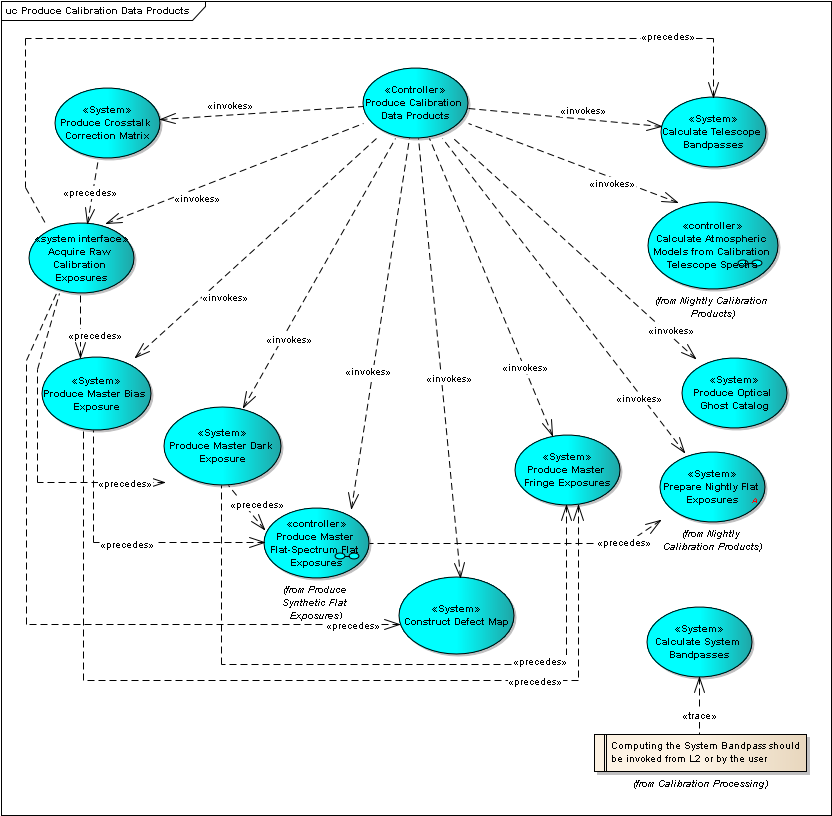
\includegraphics[angle=0,scale=0.44]{produce_calibration_data_products.png}
\caption{Calibration Products Pipeline Use Case Diagram\label{fig:cppUML}}
\end{figure}

The baseline Calibration Products Pipeline will implement all algorithms described in the Photometric Calibration Plan (\PCP). Its logical design is further described in the Calibration Processing package of the UML model (\appsUMLusecase; see also Figure~\ref{fig:cppUML} for the high-level overview).

\subsubsection{Constituent Use Cases and Diagrams}

Produce Master Fringe Exposures; Produce Master Bias Exposure; Produce Master Dark Exposure; Calculate System Bandpasses; Calculate Telescope Bandpasses; Construct Defect Map; Produce Crosstalk Correction Matrix; Produce Optical Ghost Catalog; Produce Master Pupil Ghost Exposure; Determine CCOB-derived Illumination Correction; Determine Optical Model-derived Illumination Correction; Create Master Flat-Spectrum Flat; Determine Star Raster Photometry-derived Illumination Correction; Create Master Illumination Correction; Determine Self-calibration Correction-Derived Illumination Correction; Correct Monochromatic Flats; Reduce Spectrum Exposure; Prepare Nightly Flat Exposures;

\subsubsection{Prototype Implementation}

While parts of the Calibration Products Pipeline have been prototyped by the LSST Calibration Group (see the \PCP for discussion), these have not been written using LSST Data Management software framework or coding standards. We therefore expect to transfer the know-how, and rewrite the implementation.

\clearpage

\subsection{Photometric Calibration Pipeline (\wbsPhotoCal)}

\subsubsection{Key Requirements}

The Photometric Calibration Pipeline is required to internally calibrate the relative photometric zero-points of every observation, enabling the Level 2 catalogs to reach the required SRD precision.

\subsubsection{Baseline design}

The adopted baseline algorithm is a variant of ``ubercal'' \cite{Padmanabhan08, Schlafly12}. This baseline is described in detail in the Photometric Self Calibration Design and Prototype Document (\UCAL).

\subsubsection{Constituent Use Cases and Diagrams}

Perform Global Photometric Calibration;

\subsubsection{Prototype Implementation}

Photometric Calibration Pipeline has been fully prototyped by the LSST Calibration Group to the required level of accuracy and performance (see the \UCAL document for discussion). % RHL really?  I thought that they wrote a small-scale toy version.  But I may be totally out of date.
\\

As the prototype has not been written using LSST Data Management software framework or coding standards, we assume a non-negligible refactoring and coding effort will be needed to convert it to production code in LSST Construction.

\clearpage

\subsection{Astrometric Calibration Pipeline (\wbsAstroCal)}

\subsubsection{Key Requirements}

The Astrometric Calibration Pipeline is required to calibrate the relative and absolute astrometry of the LSST survey, enabling the Level 2 catalogs to reach the required SRD precision.

\subsubsection{Baseline design}

Algorithms developed for the Photometric Calibration Pipeline (\wbsPhotoCal) will be repurposed for astrometric calibration by changing the relevant functions to minimize. This pipeline will further be aided by WCS and local astrometric registration modules developed as a component of the Single Frame Processing pipeline (\wbsSFM).
\\

Gaia standard stars will be used to fix the global astrometric system. It is likely that the existence of Gaia catalogs may make a separate Astrometric Calibration Pipeline unnecessary.

\subsubsection{Constituent Use Cases and Diagrams}

Perform Global Astrometric Calibration;

\subsubsection{Prototype Implementation}

The Astrometric Calibration Pipeline has been partially prototyped by the LSST Calibration Group, but outside of LSST Data Management software framework. We expect to transfer the know-how, and rewrite the implementation.

\clearpage

\section{Level 3 Pipelines}

\subsection{Science Pipeline Toolkit (\wbsSPT)}

\subsubsection{Key Requirements}

The Science Pipeline Toolkit shall provide the software components, services, and documentation required to construct Level 3 science pipelines out of components built for Level 1 and 2 pipelines. These pipelines shall be executable on LSST computing resources or elsewhere.

\subsubsection{Baseline design}

The baseline design assumes that Level 3 pipelines will use the same {\tt Tasks} infrastructure (see the Data Management Middleware Design document; \DMMD) as Level 1 and 2 pipelines\footnote{Another way of looking at this is that, functionally, there will be no fundamental difference between Level 2 and 3 pipelines, except for the level of privileges and access to software or hardware resources.}. Therefore, Level 3 pipelines will largely be automatically constructible as a byproduct of the overall design.
\\

The additional features unique to Level 3 involve the services to upload/download data to/from the LSST Data Access Center. The baseline for these is to build them on community standards (VOSpace).

\subsubsection{Constituent Use Cases and Diagrams}

Configure Pipeline Execution; Execute Pipeline; Incorporate User Code into Pipeline; Monitor Pipeline Execution; Science Pipeline Toolkit; Select Data to be Processed; Select Data to be Stored;

\subsubsection{Prototype Implementation}

While no explicit prototype implementation exists at this time, the majority of LSST pipeline prototypes have successfully been designed in modular and portable fashion. This has allowed a diverse set of users to customize and run the pipelines on platforms ranging from OS X laptops, to 10,000+ core clusters (e.g., BlueWaters), and to implement plugin algorithms (e.g., Kron photometry).

\clearpage

\section{Science Data Quality Analysis Pipelines}

\subsection{SDQA Pipeline (\wbsSDQAP)}

\subsubsection{Key Requirements}

SDQA Pipeline shall provide low-level data collection functionality for science data quality analysis of Level 1, 2, and Calibration Processing pipelines.
\\

In addition, SDQA Pipeline shall provide low-level data collection functionality to support software development in Construction and Operations.

\subsubsection{Baseline design}

SDQA Pipeline implementation will monitor and harvest the outputs and logs of execution of other science pipelines, computing user-defined metrics.

The metrics will be defined by extending appropriate SDQA Pipeline base classes, and configuring them in the SDQA Pipeline configuration file and/or on the command line.

The outputs of SDQA Pipeline runs will be stored into a SDQA repository (RDBMS or filesystem based).

\subsubsection{Constituent Use Cases and Diagrams}

Assess Data Quality for Nightly Processing; Assess Data Quality for Calibration Products; Assess Data Quality for Data Release;
Assess Data Quality for Nightly Processing at Archive;

\subsubsection{Prototype Implementation}

Prototype implementation of the SDQA Pipeline baseline design has been completed in LSST Final Design Phase. The existing prototype has been extensively tested with image simulation inputs, as well as real data (SDSS Stripe 82). The existing prototype will be refactored to enhance performance and flexibility in Construction.
\\

The prototype code is available in the \url{https://github.com/lsst/testing_pipeQA} git repository.

\clearpage

\subsection{SDQA Toolkit (\wbsSDQAT)}

\subsubsection{Key Requirements}

SDQA Toolkit shall.provides the visualization, analysis and monitoring capabilities for science quality data analysis. Its inputs will be provided by the SDQA Pipeline.
\\

The toolkit capabilities shall be made flexible, to provide the analyst with the ability to easily construct custom tests and analyses, and ``drill down" into various aspects of the data being analyzed.
\\

The toolkit will enable automation of tests and monitoring, and issuance of warnings when alerting thresholds are met.

\subsubsection{Baseline design}

The core of the toolkit will be designed around a pluggable Python framework generating, a web-based, interactive, visualization interface. This framework has already been implemented in the final design phase as ``pipeQA".

Standard data visualization \emph{aspects} will be realized with predefined set of web pages with tests/analyses executed on a given SDQA repository. These aspects will allow the browsing and drill-down of data collected in Data Release Production runs, or monitoring of live data (for Level 1).

Data analysts and users will be able to create new QA tests to examine particular anomalies discovered in the data. It will be possible to add these tests to the library of predefined aspects, to be executed or monitored in Level 1 and Level 2 productions.

\subsubsection{Constituent Use Cases and Diagrams}

Analyze SDQA Metrics; Correlate SDQA metric with other data; Correlate SDQA metrics; Display SDQA Metrics;

\subsubsection{Prototype Implementation}

Prototype implementation of the SDQA Toolkit has been implemented in LSST Final Design Phase. The existing prototype has been extensively tested with image simulation inputs, as well as real data (SDSS Stripe 82).
\\

The existing prototype uses a set of statically and dynamically generated pages (written in php) to display the results of data production runs. While proving invaluable for data analysis, the prototype design was found it to be difficult to extend with new analyst-developed tests. The current baseline has been defined based on this experience and will be implemented in Construction.
\\

The prototype code is available in the \url{https://github.com/lsst/testing_displayQA} git repository.

\clearpage

\section{Glossary}

\begin{description}
\item[API] Applications Programming Interface  
\item[DAC] Data Access Center
\item[DAQ] Data Acquisition
\item[DMS] Data Management System
\item[DR] Data Release.
\item[EPO] Education and Public Outreach
\item[Footprint] The set of pixels that contains flux from an object. Footprints of multiple objects may have pixels in common.
\item[FRS] Functional Requirements Specification
\item[MOPS] Moving Object Pipeline System
\item[OCS] Observatory Control System
\item[Production] A coordinated set of pipelines
\item[PSF] Point Spread Function
\item[RGB] Red-Green-Blue image, suitable for color display.
\item[SDS] Science Array DAQ Subsystem.  The system on the mountain which reads
out the data from the camera, buffers it as necessary, and supplies it
to data clients, including the DMS.
\item[SDQA] Science Data Quality Assessment.
\item[SNR] Signal-to-Noise Ratio
\item[SQL] Structured Query Language, the common language for querying relational databases.
\item[TBD] To Be Determined
\item[Visit] A pair of exposures of the same area of the sky taken in immediate
succession.  A Visit for LSST consists of a 15 second exposure, a 2
second readout time, and a second 15 second exposure.
\item[VO] Virtual Observatory
\item[VOEvent] A VO standard for disseminating information about transient events.
\item[WCS] World Coordinate System.  A bidirectional mapping between pixel- and sky-coordinates.
\end{description}

\clearpage

\begin{thebibliography}{10}

\bibitem{Ankerst99} M.~Ankerst, M.~M.~Breunig, H.-P.~Kriegel and J.~Sander,
  \textbf{OPTICS: Ordering Points To Identify the Clustering Structure},
  Proc ACM SIGMOD (1999).

\bibitem{Becker14} A.~Becker,
  \textbf{Report on Summer 2014 Production: Analysis of DCR},
  \url{https://github.com/lsst-dm/S14DCR/blob/master/report/S14report_V0-00.pdf}.

\bibitem{Bloom12} J.~S.~Bloom et al,
  \textbf{Automating discovery and classification of transients and variable stars in the synoptic survey era},
  PASP 124, 1175--1196 (2012).

\bibitem{Bosch10} J.~F.~Bosch,
  \textbf{Modeling Techniques for Measuring Galaxy Properties in Multi-Epoch Surveys},
  PhD Thesis, University of California, Davis (2011). \url{http://adsabs.harvard.edu/abs/2011PhDT.......226B}

\bibitem{Bosch13} J.~Bosch, P.~Gee, R.~Owen, M.~Juric and the LSST DM team,
  \textbf{LSST DM S13 Report: Shape measurement plans and prototypes},
  \url{https://docushare.lsstcorp.org/docushare/dsweb/ImageStoreViewer/Document-15298}

\bibitem{Huff11} E.~M.~Huff et al,
  \textbf{Seeing in the dark -- I. Multi-epoch alchemy},
  \url{http://arxiv.org/abs/1111.6958}.

\bibitem{Furusawa14} H.~Furusawa et al,
  \textbf{Hyper Suprime-Cam Survey Pipeline Description},
  \url{http://hsca.ipmu.jp/pipeline_outputs.pdf}.

\bibitem{JeeTyson11} M.~J.~Jee and J.~A.~Tyson,  \textbf{Toward
  Precision LSST Weak-Lensing Measurement. I. Impacts of Atmospheric
  Turbulence and Optical Aberration}, PASP 123, 596(2011).

\bibitem{Jee13} M.~J.~Jee, J.~A.~Tyson, M.~D.~Schneider, D.~Wittman, S.~Schmidt and S.~Hilbert,
  \textbf{Cosmic shear results from the Deep Lens Survey. I. Joint constraints on $\Omega_M$ and $\sigma_8$ with a two-dimensional analysis},
  ApJ 765 74 (2013).

\bibitem{Kubica05} J.~Kubica et al,
  \textbf{Efficiently Tracking Moving Sources in the LSST},
  Bulletin of the American Astronomical Society, 37, 1207 (2005).

\bibitem{Lang09} D.~Lang, D.~Hogg, S.~Jester and H.-W.~Rix,
  \textbf{Measuring the undetectable: Proper motions and parallaxes of very faint sources},
  AJ 137 4400--4111 (2009).

\bibitem{LuptonPhoto} R.~H.~Lupton et al,
  \textbf{SDSS Image Processing II: The \textit{Photo} Pipelines}.
  \url{http://www.astro.princeton.edu/~rhl/photo-lite.pdf}

\bibitem{Lupton05} R.~Lupton and \v{Z}.~Ivezi\'c, \textbf{Experience with SDSS: the Promise and Perils of Large Surveys},
  Astrometry in the Age of the Next Generation of Large Telescopes, ASP
  Conferences Series, Vol 338 (2005). \url{http://adsabs.harvard.edu/abs/2005ASPC..338..151L}

\bibitem{MOPS} L.~Denneau, J.~Kubica and R.~Jedicke,
   \textbf{The Pan-STARRS Moving Object Pipeline}, Astronomical Data
  Analysis Software and Systems XVI ASP Conference Series, Vol. 376,
  proceedings of the conference held 15-18 October 2006 in Tucson,
  Arizona, USA\@. Edited by Richard A. Shaw, Frank Hill and David
  J. Bell., p.257.

\bibitem{Padmanabhan08} N.~Padmanabhan et al,
  \textbf{An Improved Photometric Calibration of the Sloan Digital Sky Survey Imaging Data},
  ApJ 674 1217--1233 (2008).

\bibitem{Richards11} J.~Richards et al,
  \textbf{On Machine-learned Classification of Variable Stars with Sparse and Noisy Time-series Data},
  ApJ 733 10 (2011).

\bibitem{Schlafly12} E.~F.~Schlafly et al,
  \textbf{Photometric Calibration of the First 1.5 Years of the Pan-STARRS1 Survey},
  ApJ 756 158 (2012).

\bibitem{Szalay99} A.~S.~Szalay, A.~J.~Connolly and G.~P.~Szokoly,
  \textbf{Simultaneous Multicolor Detection of Faint Galaxies in the Hubble Deep Field},
  AJ 117 68--74 (1999).

\end{thebibliography}

\end{document}
